% Copyright (c) 2015 Daniele Masini - d.masini.it@gmail.com

\chapter{Proporzionalità e similitudine}

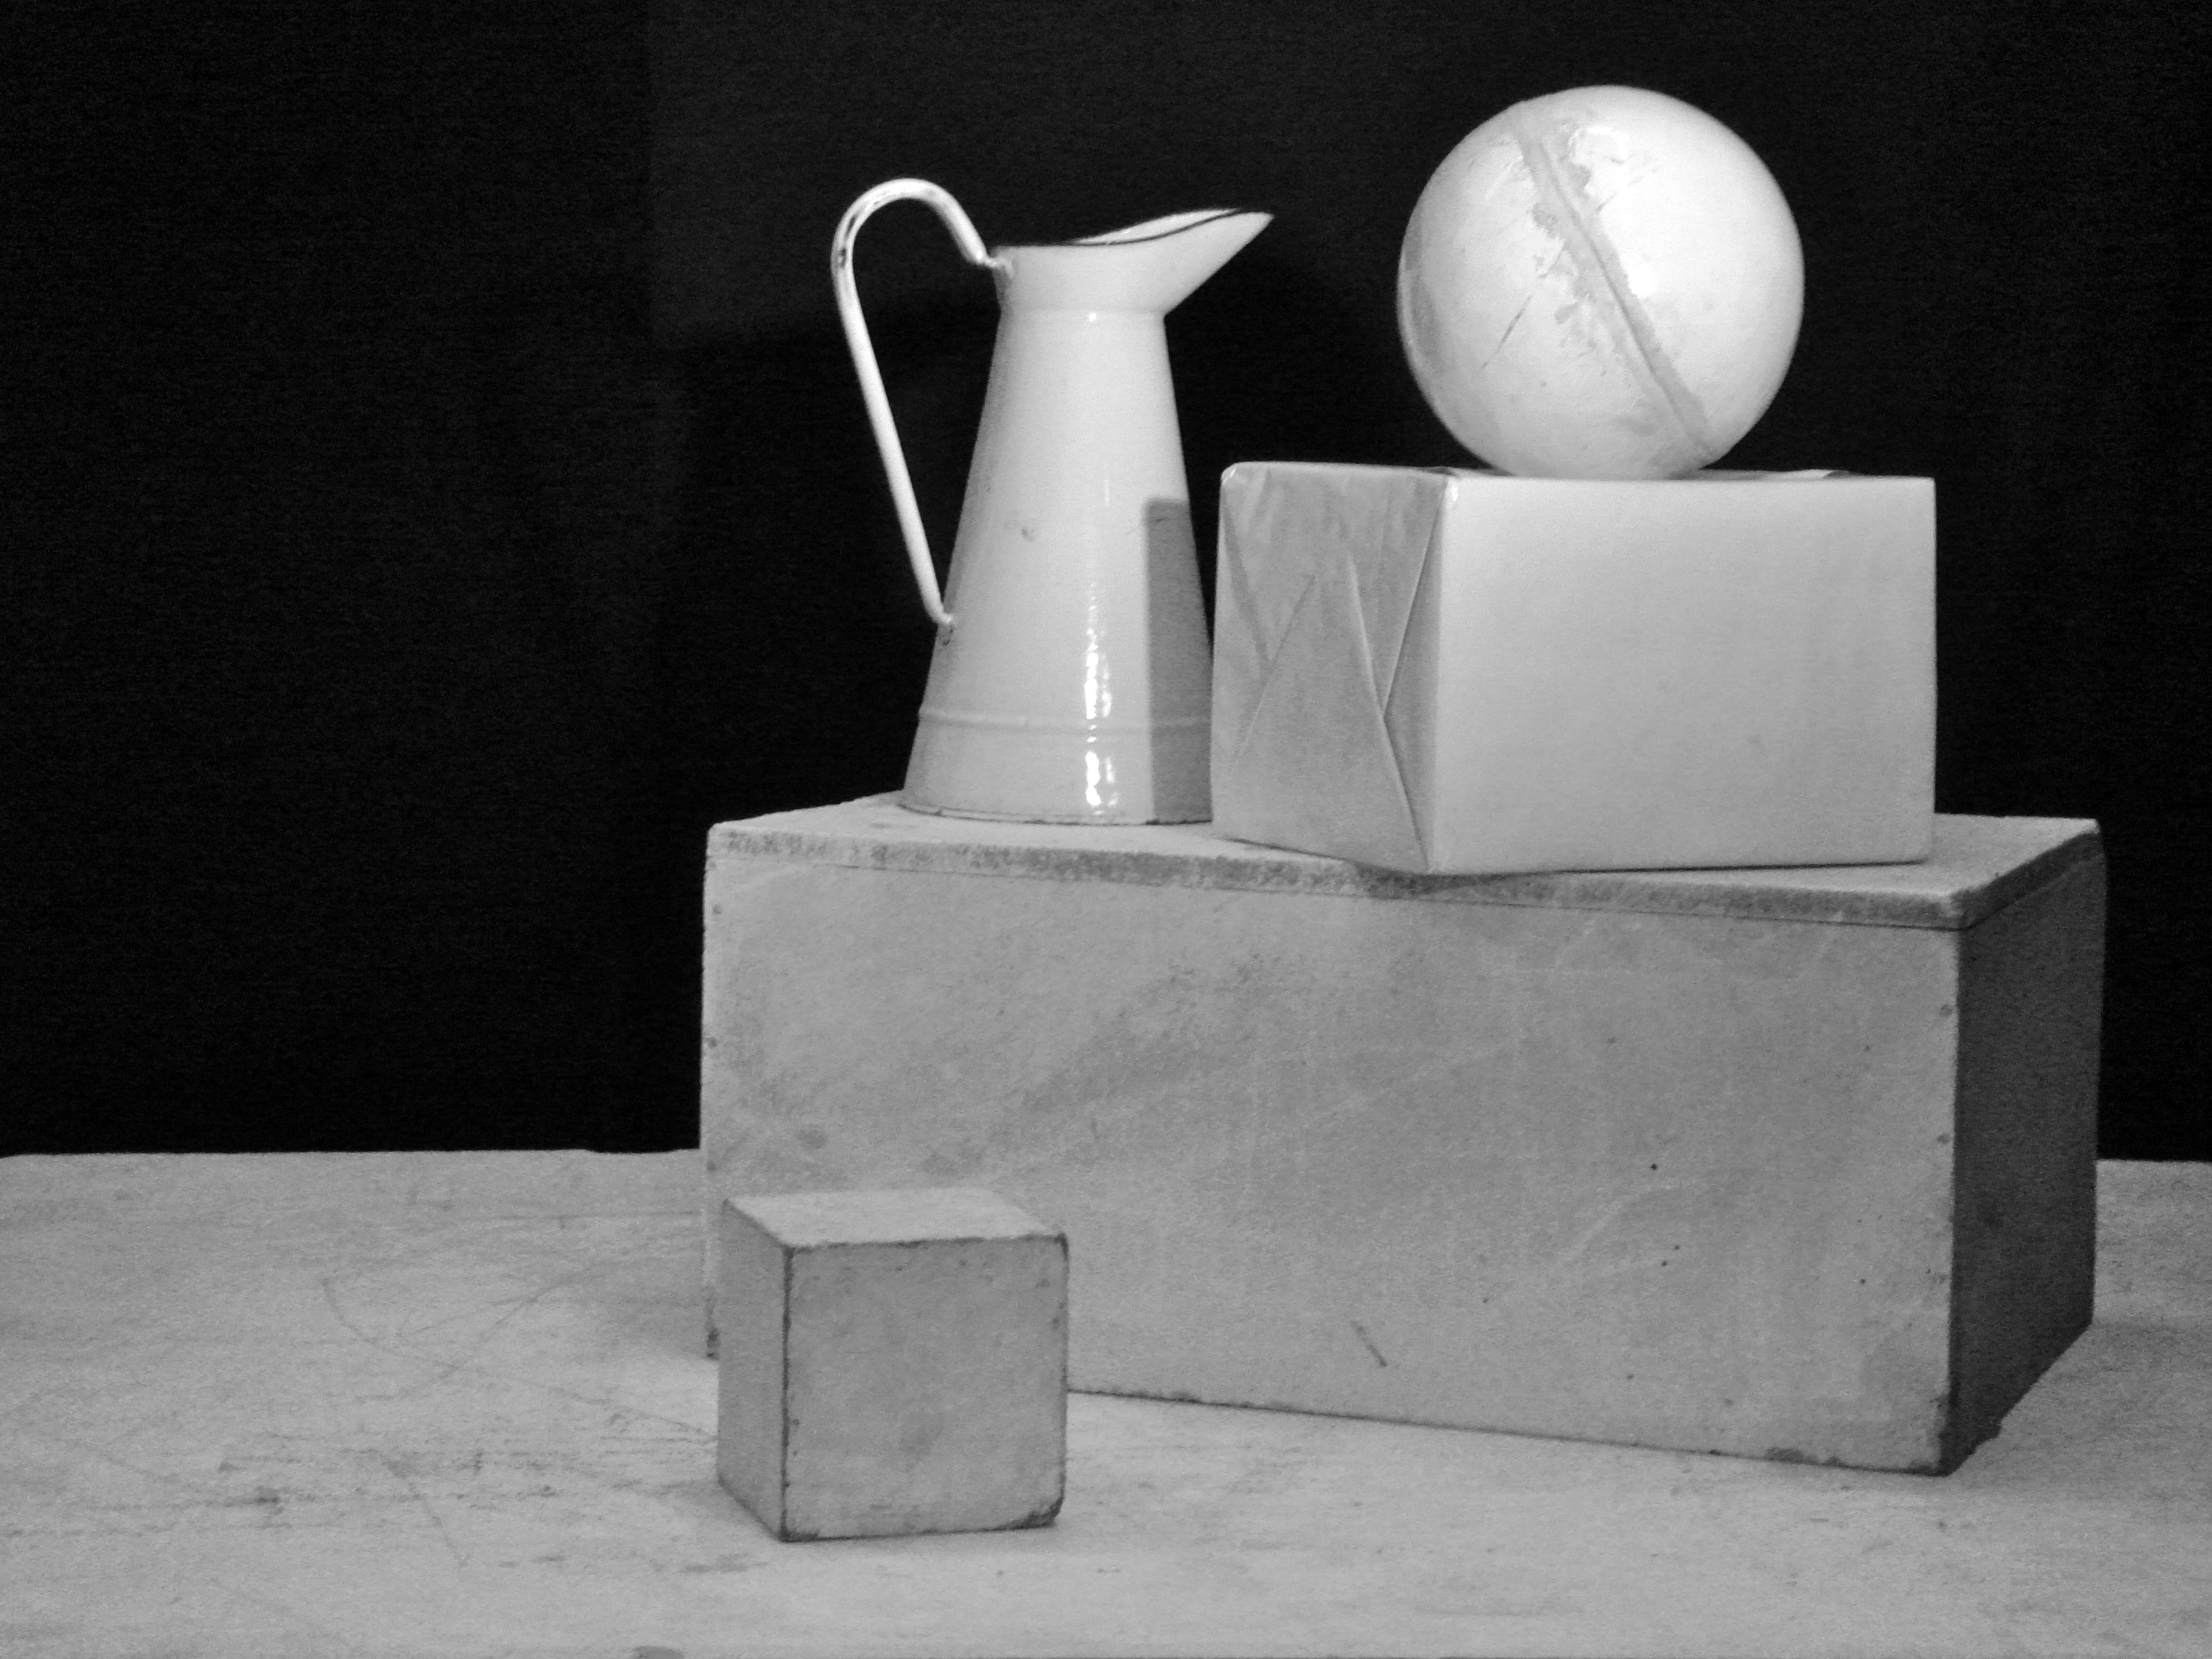
\includegraphics[width=0.95\textwidth]{\folder img/geometria.jpg}
  \begin{center}
    {\large ``Geometria''}\par
    Foto di Ram\'on Peco\par
    \url{http://www.flickr.com/photos/desdetasmania/1606257376/}\par
    Licenza: Creative Commons Attribution 2.0\par
  \end{center}
\newpage


\section{La misura}\label{sect:misura2}

\subsection{Classi di grandezze omogenee}

L'obiettivo di questo paragrafo è quello di ottenere un procedimento 
teorico per misurare alcuni enti geometrici come segmenti, angoli, 
superfici, solidi. Non è possibile invece misurare punti, rette, 
semirette.
L'operazione del \emph{misurare} consiste sostanzialmente 
nell'assegnare a una grandezza geometrica, ma non solo, un numero ben 
definito. Questo numero si ottiene confrontando la grandezza da 
misurare con una grandezza di riferimento, detta \emph{misura 
campione}. Infatti, quello che ci interessa delle grandezze è il 
fatto di poterle confrontare tra di loro per stabilire qual è la più 
grande ed eventualmente effettuarne la somma.
In generale, gli oggetti che ci circondano hanno delle 
caratteristiche: lunghezza, peso, forma, altezza, superficie, colore, 
temperatura, morbidezza, \ldots{} Alcune di queste caratteristiche 
sono confrontabili tra loro, per esempio la lunghezza di due segmenti 
o il peso di due corpi; altre non sono confrontabili. Le 
caratteristiche che si possono confrontare si dicono omogenee. Ci 
sono poi caratteristiche che sono additive, cioè si possono 
addizionare. Queste caratteristiche che hanno la peculiarità di 
essere confrontabili e sommabili si chiamano grandezze.
Nei capitoli precedenti abbiamo visto come confrontare e sommare 
segmenti, confrontare e sommare angoli. Vogliamo fare la stessa cosa 
con gli archi di circonferenza, le superfici e i volumi.
Non possiamo evidentemente confrontare e sommare punti, perché i 
punti sono tutti congruenti tra loro e sommando due punti non 
otteniamo un altro punto ma rimangono gli stessi due punti. Non 
possiamo confrontare rette perché sono tutte congruenti tra loro e non 
possiamo sommarle perché non otterremmo un'altra retta. Non possiamo 
per esempio sommare due triangoli. Né possiamo confrontare segmenti 
con angoli perché non sono grandezze omogenee, cioè non sono dello 
stesso tipo; non possiamo confrontare angoli con superfici perché 
anche questo non sono grandezze tra loro omogenee, \ldots{}
Diamo ora il concetto generale di classe di grandezze.
\begin{definizione}
Un insieme di grandezze geometriche si dice che forma una 
\emph{classe di grandezze} quando:
\begin{itemize*}
\item date due qualunque grandezze, è sempre possibile confrontarle, 
cioè stabilire se sono uguali o, in caso contrario, quali di esse sia 
la maggiore e quale la minore;
\item è sempre possibile definire un'operazione di somma tra 
grandezze che goda delle proprietà associativa e commutativa.
\end{itemize*}
Le grandezze di una stessa classe si dicono tra loro \emph{omogenee}.
\end{definizione}

A partire da questa definizione possiamo dare quella di multiplo e 
sottomultiplo.
\begin{definizione}
Data una grandezza geometrica $A$ ed un numero naturale $n$, la 
grandezza geometrica $B$ si dice \emph{multipla} di $A$ secondo il 
numero $n$ se è data dalla somma di $n$ grandezze tutte uguali ad $A$ 
e scriveremo $B=n\cdot A$. In questo caso $A$ è definita grandezza 
\emph{sottomultipla} di $B$ secondo il numero naturale $n$ e 
scriviamo $A=\dfrac{B}{n}$.
\end{definizione}

Dato un segmento $AB$ possiamo dare un significato alla scrittura 
$\dfrac{3}{2}AB$ nel seguente modo:

\begin{figure*}[!htb]
	\centering% Copyright (c) 2015 Daniele Masini - d.masini.it@gmail.com

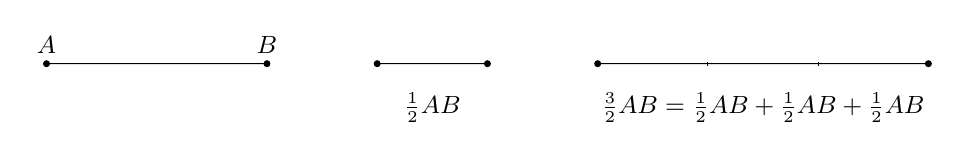
\begin{tikzpicture}[scale=0.7,font=\small,shorten line/.style={shorten >=#1,shorten <=#1}]
\usetikzlibrary{calc}

\begin{scope}
\coordinate (a) at (0,0);
\coordinate (b) at (4,0);

\draw[fill] (a) circle (1.5pt) node[above] {$A$} -- (b) circle (1.5pt) node[above] {$B$};
\end{scope}

\begin{scope}[xshift=6cm]
\coordinate (a) at (0,0);
\coordinate (b) at (2,0);

\draw[fill] (a) circle (1.5pt) -- node[below=7pt, midway] {$\frac{1}{2}AB$} (b) circle (1.5pt);
\end{scope}

\begin{scope}[xshift=10cm]
\coordinate (a) at (0,0);
\coordinate (b) at (6,0);

\foreach \x in {2,4}{%
\draw ({\x},-1pt) -- ({\x},1pt);
}

\draw[fill] (a) circle (1.5pt) -- node[below=7pt, midway] {$\frac{3}{2}AB=\frac{1}{2}AB+\frac{1}{2}AB+\frac{1}{2}AB$} (b) circle (1.5pt);

\end{scope}


\end{tikzpicture}

\end{figure*}

Il segmento $AB$ è costituito da 3 segmenti ciascuno congruente alla 
metà di $AB$.
\begin{definizione}
Due grandezze omogenee $A$ e $B$ si dicono \emph{commensurabili} 
quando esiste una terza grandezza $C$, ad esse omogenea, che è 
sottomultipla sia di $A$ che di $B$: $A=n\cdot C$, $B=m\cdot C$.
Due grandezze omogenee $A$ e $B$ si dicono \emph{incommensurabili} 
quando non esiste una terza grandezza $C$, ad esse omogenea, che sia 
sottomultipla sia di $A$ che di $B$.
\end{definizione}

L'esistenza di grandezze incommensurabili è confermata dal seguente 
teorema.
\begin{teorema}
Il lato e la diagonale di un quadrato sono grandezze incommensurabili.
\end{teorema}

\begin{figure*}[!htb]
	\centering% Copyright (c) 2015 Daniele Masini - d.masini.it@gmail.com

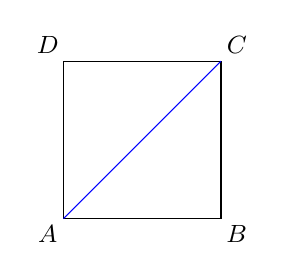
\begin{tikzpicture}[scale=2,font=\small,shorten line/.style={shorten >=#1,shorten <=#1}]
\usetikzlibrary{calc}

\begin{scope}
\draw (0,0) rectangle (1,1);
\node at ([shift={(-0.1,-0.1)}]0,0) {$A$};
\node at ([shift={(0.1,-0.1)}]1,0) {$B$};
\node at ([shift={(0.1,0.1)}]1,1) {$C$};
\node at ([shift={(-0.1,0.1)}]0,1) {$D$};
\draw[blue] (0,0) -- (1,1);

\end{scope}

\end{tikzpicture}

\end{figure*}

\begin{proof}
La dimostrazione si sviluppa per assurdo. Con riferimento alla 
figura, verifichiamo che  il lato $AB$ e la diagonale $AC$ del 
quadrato $ABCD$ sono incommensurabili.
Per assurdo, supponiamo che esista una grandezza $U$, omogenea sia al 
lato sia alla diagonale, che sia un sottomultiplo comune, cioè 
$AC=n\cdot U$ e $AB=m\cdot U$.
Per il teorema di Pitagora $AC^2=AB^2+BC^2$ e poiché $AB=BC$ si ha 
$AC^2=AB^2+AB^2=2\cdot AB^2$. Tenendo conto che $AC=n\cdot U$ e 
$AB=m\cdot U$ la formula precedente ci permette di affermare che 
$n^2\cdot U^2=2m^2\cdot U^2$. Dividendo per $U^2$ ambo i membri 
dell'uguaglianza otteniamo $n^2=2m^2$, dove $n$ e $m$ sono due numeri 
naturali. \`E abbastanza facile dimostrare che questa uguaglianza non 
può sussistere. Infatti, se $m$ è un numero pari allora $m^2$ avrà un 
numero pari di fattori uguali a 2 e quindi $2m^2$ avrà un numero 
dispari di fattori uguali a 2, ciò implica che anche $n^2$ deve avere 
un numero dispari di fattori uguali a 2; se $m$ è dispari allora 
$2m^2$ avrà un solo fattore uguale a 2 e di conseguenza non può 
essere uguale al quadrato di un numero $n$. Da cui l'assurdo che $m$ 
non può essere né pari né dispari.
\end{proof}

Storicamente, questa è stata la prima scoperta di grandezze 
incommensurabili, probabilmente dovuta al Ippaso di Metaponto, 
matematico vissuto tra Crotone e Metaponto (Calabria e Basilicata) 
nel 500 \aC circa. La tradizione dice che morì in un naufragio per 
aver rivelato la scoperta dell'esistenza delle grandezze 
incommensurabili, in contrasto con il pensiero del maestro Pitagora.
Siano $A$ e $B$ due grandezze omogenee commensurabili, sia $C$ la 
grandezza sottomultipla in comune, si avrà $A=n\cdot C$ e $B=m\cdot 
C$. Da cui $C=\dfrac{1}{n}A$ e $C=\dfrac{1}{m}B$. Dal confronto si ha 
$\dfrac{1}{n}A=\dfrac{1}{m}B$ da cui $A=\dfrac{n}{m}B$.

\begin{definizione}
Si dice \emph{rapporto di due grandezze omogenee} $A$ e $B$ il numero 
razionale $\dfrac{n}{m}$ tale che $A=\dfrac{n}{m}B$.
\end{definizione}
Occorre supporre la validità dei seguenti postulati.\vspace{8pt}

\noindent \emph{Postulato della divisibilità.} Ogni grandezza 
geometrica è sempre divisibile in un numero qualunque di 
parti.\vspace{8pt}

\noindent \emph{Postulato di Eudosso-Archimede.} Date due grandezze 
omogenee disuguali esiste sempre una grandezza multipla della minore 
che supera la maggiore.\vspace{8pt}

Possiamo dare ora la definizione di misura di un segmento rispetto a 
un altro, nel caso in cui i due segmenti sono commensurabili.
\begin{definizione}
Date due grandezze $A$ e $U$ tra loro commensurabili si definisce 
\emph{misura di $A$ rispetto a $U$} il numero razionale 
$\dfrac{m}{n}$ per il quale $A=\dfrac{m}{n}U$. La grandezza $U$ viene 
detta \emph{unità di misura}.
\end{definizione}

Per le definizioni precedenti, la misura di $U$ rispetto a se stessa 
è evidentemente 1.

Solitamente si usa come unità di misura delle lunghezze il metro 
(indicato con il simbolo m), con il suo multipli (decametro dam, 
ettometro hm, chilometro km, \ldots{}) ed i suoi sottomultipli 
(decimetro dm, centimetro cm, millimetro mm, \ldots{}). Per misurare 
gli angoli si usa il grado che è la 360\textsuperscript{a} parte 
dell'angolo giro. Per misurare le superfici si usa come unità di 
superficie quella di un quadrato di lato 1~m (metro quadrato, 
indicato con il simbolo m\textsuperscript{2}) con i suoi multipli e 
sottomultipli. Per misurare i solidi si usa il volume di un cubo di 
lato 1~m (metro cubo, indicato con il simbolo m\textsuperscript{3}).

Per quanto riguarda la scrittura delle misure, in Italia valgono le 
seguenti norme: l'unità di misura si scrive sempre dopo il numero che 
la indica, tranne per le misure monetarie: si scrive 12~m e non m~12; 
si scrive \officialeuro~12 e non 12~\officialeuro. L'unità di misura 
non è mai seguita dal puntino e non va mai espressa al plurale.

\`E possibile estendere la definizione di rapporto e la conseguente 
definizione di misura anche per la grandezze tra loro 
incommensurabili, come per esempio lato e diagonale dello stesso 
quadrato. Il percorso però è più lungo e complesso, poiché il 
rapporto tra due grandezze commensurabili è sempre un numero razionale 
mentre il rapporto tra due grandezze incommensurabili non è un numero 
razionale.

Partiamo dalla definizione di classi contigue.
\begin{definizione}
Due classi di grandezze omogenee si dicono \emph{contigue} se godono 
delle seguenti proprietà:
\begin{itemize*}
\item sono \emph{separate}: ogni grandezza della prima classe è 
minore di ogni grandezza della seconda classe. Vale a questo proposito 
il \emph{postulato della continuità}, secondo il quale due classi di 
grandezze separate ammettono almeno un elemento separatore (ne esiste 
sicuramente uno, ma potrebbero anche essercene infiniti), cioè una 
grandezza che sia maggiore (o uguale) di ogni grandezza della prima 
classe e minore (o uguale) di ogni grandezza della seconda.
\item godono della \emph{proprietà dell'avvicinamento indefinito}: 
presa una grandezza $\epsilon$, piccola a piacere, omogenea a quelle 
date, esiste sempre una grandezza della seconda classe ed una della 
prima la cui differenza sia minore di $\epsilon$.
\end{itemize*}
\end{definizione}

Per due classi di grandezze contigue vale l'\emph{assioma di Cantor}: 
due classi di grandezze contigue ammettono uno e un solo elemento 
separatore.

Basandoci sul concetto di contiguità possiamo a questo punto definire 
un qualunque \emph{numero irrazionale} come l'unico elemento 
separatore tra due classi contigue di numeri razionali; nella prima 
classe mettiamo tutti i numeri che approssimano il numero irrazionale 
per difetto e nella seconda quelli che lo approssimano per eccesso.

Prendendo come esempio il numero irrazionale $\sqrt{2}$ le due classi 
sono:
\[A: 1\quad \np{1,4}\quad \np{1,41}\quad \np{1,414}\quad 
\np{1,4142}\quad \ldots{}\]
\[B: 2\quad \np{1,5}\quad \np{1,42}\quad \np{1,415}\quad 
\np{1,4143}\quad \ldots{}\]
Si può osservare che le due successioni sono separate, in quanto ogni 
numero della prima è minore di ogni numero della seconda, inoltre 
godono della proprietà dell'avvicinamento indefinito, in quanto è 
sempre possibile trovare un numero razionale appartenente ad $A$ ed 
uno appartenente a $B$ la cui differenza sia minore di un qualsiasi 
numero $\epsilon$, per quanto piccolo questo si prenda.
Quindi, per l'assioma di Cantor, esiste ed è unico l'unico elemento 
separatore di queste due successioni; possiamo identificare questo 
numero con la coppia di successioni e scrivere: $\sqrt{2} = (A\text{, 
}B)$.

Questa definizione vale non solo per i numeri irrazionali, ma anche 
per quelli razionali. Per esempio, la frazione $\dfrac{15}{4}=3,75$ è 
definita dalle classi contigue:
\[A: 3\quad \np{3,7}\quad \np{3,74}\quad \np{3,749}\quad 
\np{3,7499}\quad \ldots{}\]
\[B: 4\quad \np{3,8}\quad \np{3,75}\quad \np{3,750}\quad 
\np{3,7501}\quad \ldots{}\]

Possiamo naturalmente definire in questo modo anche i numeri interi. 
Per esempio 5 è l'elemento separatore delle classi:
\[A: 4\quad \np{4,9}\quad \np{4,99}\quad \np{4,999}\quad 
\np{4,9999}\quad \ldots{}\]
\[B: 6\quad \np{5,1}\quad \np{5,01}\quad \np{5,001}\quad 
\np{5,0001}\quad \ldots{}\]

Concludiamo quindi affermando che un qualunque numero reale $r$ può 
essere definito come l'elemento separatore di una coppia di classi 
numeriche contigue.

\pagebreak

I numeri reali sono pertanto il raggruppamento di numeri razionali e 
irrazionali:

\begin{figure*}[!htb]
	\centering% Copyright (c) 2015 Daniele Masini - d.masini.it@gmail.com

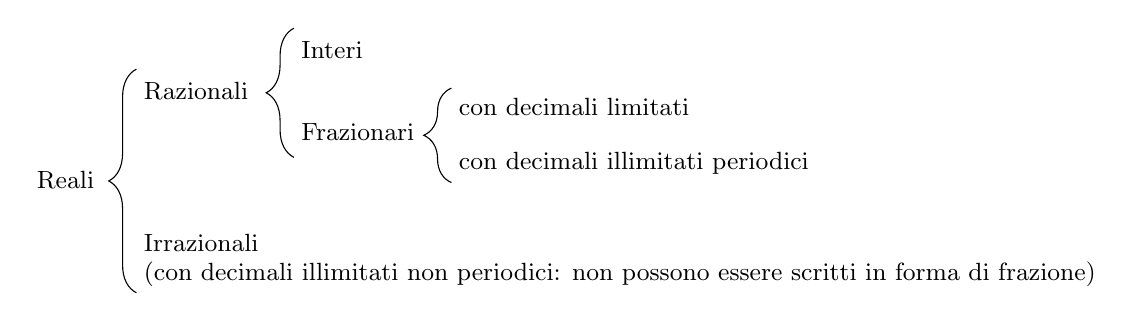
\begin{tikzpicture}[scale=0.8,font=\small]
\usetikzlibrary{calc, decorations.pathreplacing}

\begin{scope}
\node[right] at (0.3,0) {Reali};
\node[right] at (2,1.4) {Razionali};
\node[right] at (2,-1) {Irrazionali};
\node[right] at (2,-1.5) {(con decimali illimitati non periodici: non possono essere scritti in forma di frazione)};
\node[right] at (4.5,2.05) {Interi};
\node[right] at (4.5,0.75) {Frazionari};
\node[right] at (7,1.15) {con decimali limitati};
\node[right] at (7,0.25) {con decimali illimitati periodici};

\draw [decorate,decoration={brace,amplitude=10pt},xshift=1pt,yshift=0pt] (2,-1.8) -- (2,1.75);
\draw [decorate,decoration={brace,amplitude=10pt},xshift=1pt,yshift=0pt] (4.5,0.35) -- (4.5,2.40);
\draw [decorate,decoration={brace,amplitude=10pt},xshift=1pt,yshift=0pt] (7,-0.05) -- (7,1.45);

\end{scope}

\end{tikzpicture}

\end{figure*}

Passiamo ora a definire la misura delle grandezze incommensurabili.
Date le lunghezze incommensurabili AB e CD, poniamo
\[A=\left\{\dfrac{m}{n}\in\insQ^+\mid\dfrac{m}{n}CD<AB\right\}
\qquad\text{e} \qquad 
B=\left\{\dfrac{m}{n}\in\insQ^+\mid\dfrac{m}{n}CD>AB\right\}.\]
Si dimostra che la coppia $(A\text{, }B)$ è una coppia di classi 
contigue di $\insQ^+$. In maniera intuitiva possiamo dire che $A$ 
contiene i valori approssimati per difetto e $B$ contiene i valori 
approssimati per eccesso del rapporto $\dfrac{m}{n}$.
Chiamiamo \emph{rapporto fra le lunghezze incommensurabili} $AB$ e 
$CD$ il numero irrazionale dato dalle classi contigue $(A\text{, }B)$.


\section{Proporzionalità tra grandezze}\label{sect:proporzioni}

\begin{definizione}
Date quattro grandezze $A$, $B$, $C$ e $D$, le prime due omogenee tra 
loro così come le ultime due, queste formano una \emph{proporzione} 
se il rapporto delle prime due è uguale al rapporto delle ultime due. 
Si scrive
\begin{empheq}[box=\fbox]{equation*}
A : B = C : D
\end{empheq}
e si legge ``$A$ sta a $B$ come $C$ sta a $D$''.
\end{definizione}

\begin{definizione}
In una proporzione
\begin{itemize*}
\item il primo ed il terzo termine ($A$ e $C$) si chiamano 
\emph{antecedenti};
\item il secondo ed il quarto termine ($B$ e $D$) si chiamano 
\emph{conseguenti};
\item $B$ e $C$ si chiamano \emph{medi};
\item $A$ e $D$ si chiamano \emph{estremi};
\item la grandezza $D$ si chiama \emph{quarta proporzionale}.
\end{itemize*}
\end{definizione}

\begin{definizione}
Se in una proporzione tra grandezze tutte omogenee i medi sono uguali 
tra loro $A : B = B : C$, la proporzione si dice \emph{continua}, la 
grandezza $B$ si chiama \emph{media proporzionale} e la grandezza $C$ 
si dice \emph{terza proporzionale}.
\end{definizione}

\begin{teorema}[fondamentale delle proporzioni]\label{teo:fond_prop}
Condizione necessaria e sufficiente affinché quattro grandezze siano 
in proporzione è che siano in proporzione le loro misure.
\end{teorema}

\begin{proof}
Siano $A$ e $B$ due grandezze omogenee, $a$ e $b$ le loro misure 
rispetto ad un'unità di misura omogenea ad $A$ e $B$; $C$ e $D$ due 
grandezze anch'esse omogenee tra loro e $c$ e $d$ le loro misure 
rispetto ad un'unità di misura omogenea a $C$ e $D$.
\begin{enumerate*}
\item (condizione necessaria $\Rightarrow$)\\
Dimostriamo innanzitutto che la condizione è necessaria: supposto che 
le quattro grandezze siano in proporzione, dimostriamo che sono in 
proporzione le loro misure.\\
Ipotesi: $A : B = C : D$ \tab Tesi: $a : b = c : d$.\\
Applicando il teorema secondo cui il rapporto tra due grandezze è 
uguale al quoziente delle loro misure, avremo 
$\dfrac{A}{B}=\dfrac{a}{b}$ e $\dfrac{C}{D}=\dfrac{c}{d}$. Ma per 
ipotesi $\dfrac{A}{B}=\dfrac{C}{D}$ e quindi, per la proprietà 
transitiva dell'uguaglianza, avremo che $\dfrac{a}{b}=\dfrac{c}{d}$, 
che si può anche scrivere nella forma $a : b = c : d$.

\item (condizione sufficiente $\Leftarrow$)\\
Dimostriamo ora che la condizione è sufficiente.\\
Ipotesi: $a : b = c : d$\tab Tesi: $A : B = C : D$.\\
Sempre dal teorema citato precedentemente, poiché 
$\dfrac{A}{B}=\dfrac{a}{b}$ e $\dfrac{C}{D}=\dfrac{c}{d}$, per la 
proprietà transitiva dell'uguaglianza avremo che 
$\dfrac{a}{b}=\dfrac{C}{D}$, vale a dire $A : B = C : D$.
\end{enumerate*}
\end{proof}

Ricordiamo che per la proporzionalità tra numeri vale la seguente
\begin{proprieta}
Condizione necessaria e sufficiente affinché quattro numeri siano in 
proporzione è che il prodotto dei medi sia uguale al prodotto degli 
estremi.
\end{proprieta}

\subsection{Proprietà delle proporzioni}

Grazie al teorema fondamentale delle proporzioni 
(teorema~\ref{teo:fond_prop}) possiamo trasferire le proprietà delle 
proporzioni tra numeri alle proporzioni tra grandezze.

\begin{enumerate*}
\item \textbf{Proprietà dell'invertire}\\
Scambiando ogni antecedente col proprio conseguente otteniamo una 
nuova proporzione equivalente alla precedente.
\[A : B = C : D \:\Rightarrow\: B : A = D : C.\]

\item \textbf{Proprietà del permutare}
Se le quattro grandezze sono tutte omogenee, possiamo scambiare tra 
loro i medi o gli estremi, ed otterremo sempre una nuova proporzione 
equivalente alla precedente.
\[A : B = C : D \:\Rightarrow\: D : B = C : A.\]

\item \textbf{Proprietà del comporre}
La somma delle prime due grandezze sta alla prima (o alla seconda) 
grandezza come la somma delle altre due sta alla terza (o alla 
quarta).
\[A : B = C : D \:\Rightarrow\: (A + B) : A = (C + D) : C\]
\noindent e
\[A : B = C : D \:\Rightarrow\: (A + B) : B = (C + D) : D\]

\item \textbf{Proprietà dello scomporre}
La differenza tra la prima e la seconda grandezza sta alla prima (o 
alla seconda) grandezza come la differenza tra le altre due sta alla 
terza (o alla quarta). Questa proprietà richiede che ogni antecedente 
sia  maggiore del proprio conseguente. Se dunque $A > B$ e $C > D$ 
avremo che
\[A : B = C : D \:\Rightarrow\: (A - B) : A = (C - D) : C\]
\noindent e
\[A : B = C : D \:\Rightarrow\: (A - B) : B = (C - D) : D\]
\end{enumerate*}

In riferimento alla disuguaglianza precedente, va precisato che se 
quattro grandezze sono in proporzione, tra antecedenti e conseguenti 
intercorre sempre la stessa relazione, vale a dire che se la prima 
grandezza è uguale, maggiore o minore della seconda, anche la terza 
sarà uguale, maggiore o minore della quarta.

\begin{teorema}[della quarta proporzionale]
Date tre grandezze $A$, $B$ e $C$, con $A$ e $B$ omogenee tra loro, 
esiste ed è unica una grandezza $D$, omogenea alla terza, che con le 
tre date formi una proporzione.
\end{teorema}

\begin{proof}
Siano $A$, $B$ e $C$ tre grandezze, le prime due omogenee tra loro. 
Supponiamo che esista una quarta grandezza $X$, omogenea a $C$, tale 
che valga la proporzione $A : B = C : X$.
Sostituendo alle grandezze le loro misure, per il teorema 
fondamentale delle proporzioni (\ref{teo:fond_prop}) dovrà essere $a : 
b = c : x$.
Applichiamo ora la proprietà fondamentale delle proporzioni 
numeriche, uguagliando il prodotto dei medi a quello degli estremi 
$ax = bc$.
Risolvendo l'equazione in $x$ otteniamo $x = \dfrac{bc}{a}$, e poiché 
$a$, $b$ e $c$ sono diversi da zero (e positivi), in quanto misure di 
grandezze geometriche, quest'equazione avrà come soluzione uno e un 
solo numero reale (positivo), in quanto la soluzione di un'equazione 
di primo grado, se esiste, è unica.
Questo numero reale sarà quindi la misura della quarta grandezza $X$, 
e poiché tra grandezze omogenee ad ogni numero reale corrisponde una 
e una sola grandezza, questa quarta proporzionale esiste ed è unica.
\end{proof}

\subsection{Grandezze direttamente e inversamente proporzionali}

Consideriamo due classi di grandezze
\[A\text{,}\quad B\text{,}\quad C\text{,}\quad D\text{,}\quad 
\ldots{}\]
\[A'\text{,}\quad B'\text{,}\quad C'\text{,}\quad D'\text{,}\quad 
\ldots{}\]
Queste due classi si dicono in \emph{corrispondenza biunivoca} quando 
ad ogni grandezza della prima classe corrisponde una e una sola 
grandezza della seconda e viceversa.
Le grandezze $A$ e $A'$, $B$ e $B'$, $C$ e $C'$, $D$ e $D'$, \ldots{} 
si dicono \emph{corrispondenti}.

Le grandezze di queste due classi si dicono \emph{direttamente 
proporzionali} quando il rapporto di due grandezze qualunque della 
prima classe è uguale al rapporto delle due grandezze corrispondenti 
della seconda classe, cioè quando valgono le proporzioni
\[A : B = A' : B'\qquad\qquad A : C = A' : C'\qquad\qquad B : C = B' 
: C'\qquad\qquad\ldots{}\]
Se poi le grandezze della prima classe sono omogenee con quelle della 
seconda, allora possiamo permutare i medi
\[A : A' = B : B'\qquad\qquad A : A' = C : C'\qquad\qquad B : B' = C 
: C'\qquad\qquad\ldots{}\]
e, applicando la proprietà transitiva dell'uguaglianza, otteniamo
\[A : A' = B : B' = C : C' = \ldots{} = k\]
da cui segue che \emph{il rapporto tra due grandezze corrispondenti è 
costante}. Questo rapporto costante è un numero detto \emph{costante 
di proporzionalità}.

Se le grandezze della prima classe non fossero omogenee con quelle 
della seconda, dovremmo passare dalla proporzionalità tra le 
grandezze a quella tra le loro misure (reso sempre possibile dal 
teorema fondamentale delle proporzioni -- \ref{teo:fond_prop}), ed in 
questo caso sarebbe il rapporto tra le loro misure ad essere costante.

Per determinare se due classi di grandezze sono direttamente 
proporzionali si applica il seguente teorema
\begin{teorema}\label{teo:6.1}
Condizione necessaria e sufficiente affinché due classi di grandezze 
in corrispondenza biunivoca siano direttamente proporzionali è che
\begin{itemize*}
\item a grandezze uguali della prima classe corrispondano grandezze 
uguali della seconda;
\item alla somma di due o più grandezze della prima classe 
corrisponda la somma delle grandezze corrispondenti della seconda 
classe.
\end{itemize*}
\end{teorema}

\begin{proof}~\\
\begin{itemize*}
\item (condizione necessaria $\Rightarrow$)\\
Dimostriamo che la condizione è necessaria, cioè che se le grandezze 
sono proporzionali, allora devono valere le due proprietà.
Dette $A$ e $B$ due grandezze della prima classe, e $A'$, $B'$ le 
grandezze corrispondenti della seconda classe, per ipotesi avremo $A 
: B = A' : B'$.
Se $A=B$, il loro rapporto è 1, e tale deve essere il rapporto tra 
$A'$ e $B'$, da cui segue $A' = B'$.
Quindi la prima proprietà è verificata.
Applichiamo ora alla proporzione data la proprietà del comporre $(A + 
B) : A = (A' + B') : A'$.
Se $C$ è la grandezza della prima classe tale che $C = A + B$, 
sostituendo nella proporzione avremo:
$C : A = (A' + B') : A'$.
Se $C'$ è la grandezza che corrisponde a $C$, poiché per ipotesi le 
due classi di grandezze sono direttamente proporzionali, dovrà valere 
anche la seguente proporzione $(A + B) : A = C' : A'$, e per 
l'unicità della quarta proporzionale dovrà essere $C' = A' + B'$.
Anche la seconda proprietà risulta dunque verificata.
\item (condizione sufficiente $\Leftarrow$)\\
Dimostriamo ora che la condizione è sufficiente:  se valgono le due 
proprietà, le due classi di grandezze sono direttamente proporzionali.
Consideriamo due grandezze qualunque della prima classe $A$ e $B$; 
possono essere uguali o disuguali.
Se $A = B$, allora per la prima proprietà sarà pure $A' = B'$; poiché 
$A : B = 1$ e $A' : B' = 1$, per la proprietà transitiva 
dell'uguaglianza dovrà essere $A : B = A' : B'$, quindi il rapporto 
tra due grandezze qualunque della prima classe è uguale al rapporto 
delle grandezze corrispondenti della seconda, e perciò le due classi 
di grandezze sono direttamente proporzionali.
Supponiamo ora $A$ e $B$ disuguali, sia ad esempio $A > B$. Questo 
vuol dire che esiste una terza grandezza $C$ tale che $A = B + C$. 
Per la seconda proprietà a $B + C$ corrisponde $B' + C'$ e per la 
prima proprietà ad $A = B + C$ corrisponde $A' = B' + C'$, da cui si 
deduce che $A' > B'$.
Analogamente si dimostra che se $A < B$, allora $A' < B'$.

Sempre per la seconda proprietà, moltiplicando le grandezze per uno 
stesso numero naturale avremo che ad $n\cdot A$ corrisponderà $n\cdot 
A'$ e ad $m\cdot B$ corrisponderà $m\cdot B'$. Per quanto premesso, 
avremo che se $n\cdot A = m\cdot B$, sarà anche $n\cdot A' = m\cdot 
B'$; se $n\cdot A > m\cdot B$, sarà anche $n\cdot A' > m\cdot B'$ ed 
infine, se $n\cdot A < m\cdot B$, ne deriverà che $n\cdot A' < m\cdot 
B'$.
Questo vuol dire che, andando a costruire il rapporto tra le 
grandezze, avremo
\[\dfrac{A}{B} = \dfrac{m}{n} \:\Rightarrow\: \dfrac{A'}{B'} = 
\dfrac{m}{n}\qquad \dfrac{A}{B} > \dfrac{m}{n} \:\Rightarrow\: 
\dfrac{A'}{B'} > \dfrac{m}{n}\qquad \dfrac{A}{B} < \dfrac{m}{n} 
\:\Rightarrow\: \dfrac{A'}{B'} < \dfrac{m}{n}.\]
 
Dunque i rapporti $\dfrac{A}{B}$ e $\dfrac{A'}{B'}$ ammettono gli 
stessi valori approssimati per difetto o per eccesso, e quindi questi 
rapporti rappresentano lo stesso numero reale. Per cui, concludendo, 
si ha $A : B = A' : B'$.
\end{itemize*}
\end{proof}

\subsection{Grandezze inversamente proporzionali}

Le grandezze di due classi in corrispondenza biunivoca si dicono 
\emph{inversamente proporzionali} quando il rapporto di due grandezze 
qualunque della prima classe è uguale al rapporto inverso delle due 
grandezze corrispondenti della seconda classe, cioè quando valgono le 
proporzioni
\[A : B = B' : A'\qquad\qquad A : C = C' : A'\qquad\qquad B : C = C' 
: B'\qquad\qquad \ldots{}\]
Se dalla proporzionalità tra le grandezze passiamo a quella tra le 
loro misure avremo
\[a : b = b' : a'\qquad\qquad a : c = c' : a'\qquad\qquad b : c = c' 
: b'\qquad\qquad \ldots{}\]
Applicando la proprietà fondamentale della proporzionalità tra numeri 
(il prodotto dei medi è uguale al prodotto degli estremi) avremo
\[aa' = bb'\qquad\qquad aa' = cc'\qquad\qquad bb' = cc'\qquad\qquad 
\ldots{}\]
e, applicando la proprietà transitiva dell'uguaglianza
\[aa' = bb' = cc' = \ldots{} =k\]
da cui segue che \emph{il prodotto tra le misure di due grandezze 
corrispondenti è costante}. Anche in questo caso il prodotto costante 
è un numero detto \emph{costante di proporzionalità}.

\subsubsection{Teoremi su particolari classi di grandezze 
direttamente proporzionali}

\begin{teorema}\label{teo:6.2}
I rettangoli aventi altezze congruenti sono proporzionali alle 
rispettive basi.
\end{teorema}

\begin{figure*}[!htb]
	\centering% Copyright (c) 2015 Daniele Masini - d.masini.it@gmail.com

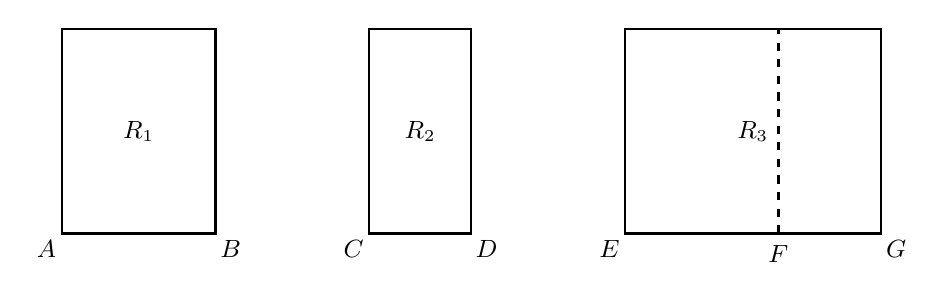
\begin{tikzpicture}[scale=1.3,font=\small,shorten line/.style={shorten >=#1,shorten <=#1}]
\usetikzlibrary{calc}

\begin{scope}
\draw[thick] (0,0) rectangle (1.5,2);
\node at (0.75,1) {$R_1$};
\node at ([shift={(-0.15,-0.15)}]0,0) {$A$};
\node at ([shift={(0.15,-0.15)}]1.5,0) {$B$};
\end{scope}

\begin{scope}[xshift=3cm]
\draw[thick] (0,0) rectangle (1,2);
\node at (0.5,1) {$R_2$};
\node at ([shift={(-0.15,-0.15)}]0,0) {$C$};
\node at ([shift={(0.15,-0.15)}]1,0) {$D$};
\end{scope}

\begin{scope}[xshift=5.5cm]
\draw[thick] (0,0) rectangle (2.5,2);
\node at (1.25,1) {$R_3$};
\node at ([shift={(-0.15,-0.15)}]0,0) {$E$};
\node at ([shift={(0.15,-0.15)}]2.5,0) {$G$};
\draw[thick, dashed] (1.5,0) -- (1.5,2);
\node at ([shift={(0,-0.2)}]1.5,0) {$F$};
\end{scope}

\end{tikzpicture}
	
\end{figure*}

\begin{proof}
Consideriamo la classe di grandezze costituita da tutti i rettangoli 
con altezze congruenti e la classe costituita dalle rispettive basi. 
Queste due classi sono in corrispondenza biunivoca, in quanto ad ogni 
rettangolo corrisponde una ed una sola base e viceversa.
Per dimostrare che queste due classi sono direttamente proporzionali 
applichiamo il teorema~\ref{teo:6.1} dimostrato precedentemente. 
Dobbiamo cioè verificare che siano soddisfatte le due proprietà.

\emph{Prima proprietà: a grandezze uguali della prima classe devono 
corrispondere grandezze uguali della seconda.}\\
Si nota facilmente che questa proprietà è sempre verificata, in 
quanto se si suppone che $AB = CD$, allora anche i rettangoli che 
hanno questi segmenti come base, avendo le altezze congruenti, 
saranno sicuramente congruenti.

\emph{Seconda proprietà: ad un segmento che sia la somma di due 
segmenti deve corrispondere un rettangolo che sia la somma di due 
rettangoli aventi quei segmenti come base.}\\
Supponiamo infatti $EG =  AB + CD$; prendiamo su $EG$ il punto $F$ 
che divida il segmento in due parti: $EF=AB$, $FG=CD$. Tracciando la 
perpendicolare in $F$ ad $EG$, questa divide il rettangolo $R_3$ in 
due rettangoli rispettivamente congruenti ad $R_1$ e ad $R_2$, e 
quindi $R_3= R_1+R_2$.

Poiché dunque valgono le due proprietà richieste dal teorema, avremo 
che $R_1 : R_2 = AB : CD$, 
$R_2 : R_3 = CD  : EG$, \ldots{} e quindi le due classi di grandezze 
sono direttamente proporzionali.
\end{proof}

In modo analogo si dimostra che:
\begin{itemize*}
\item \emph{I rettangoli aventi basi congruenti sono direttamente 
proporzionali alle rispettive altezze.}
\item \emph{Gli archi di una stessa circonferenza sono direttamente 
proporzionali ai corrispondenti angoli al centro.}
\end{itemize*}


\section{Teorema di Talete, caso generale}\label{sect:talete_generale}

\begin{teorema}[di Talete]
Un fascio di rette parallele determina su due trasversali classi di 
segmenti direttamente proporzionali.
\end{teorema}

\begin{proof}
Assumiamo come ipotesi di avere quattro rette parallele $a$, $b$, $c$ 
e $d$. Dimostriamo che sono proporzione i segmenti 
$A_1B_1 : A_2B_2 = B_1C_1 : B_2C_2 = A_1C_1 : A_2C_2 = B_1D_1 : 
B_2D_2$.

\begin{figure*}[!htb]
	\centering% Copyright (c) 2015 Daniele Masini - d.masini.it@gmail.com

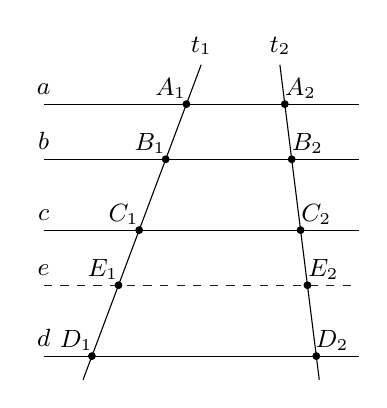
\begin{tikzpicture}[scale=1,font=\small]
\usetikzlibrary{calc}

\begin{scope}
\coordinate (a1) at (0,0);
\coordinate (a2) at (4,0);
\coordinate (b1) at (0,-.7);
\coordinate (b2) at (4,-.7);
\coordinate (c1) at (0,-1.6);
\coordinate (c2) at (4,-1.6);
\coordinate (d1) at (0,-3.2);
\coordinate (d2) at (4,-3.2);
\coordinate (e1) at (0,-2.3);
\coordinate (e2) at (4,-2.3);
\coordinate (t11) at (2,0.5);
\coordinate (t12) at (0.5,-3.5);
\coordinate (t21) at (3,0.5);
\coordinate (t22) at (3.5,-3.5);
\coordinate (A1) at (intersection of a1--a2 and t11--t12);
\coordinate (A2) at (intersection of a1--a2 and t21--t22);
\coordinate (B1) at (intersection of b1--b2 and t11--t12);
\coordinate (B2) at (intersection of b1--b2 and t21--t22);
\coordinate (C1) at (intersection of c1--c2 and t11--t12);
\coordinate (C2) at (intersection of c1--c2 and t21--t22);
\coordinate (D1) at (intersection of d1--d2 and t11--t12);
\coordinate (D2) at (intersection of d1--d2 and t21--t22);
\coordinate (E1) at (intersection of e1--e2 and t11--t12);
\coordinate (E2) at (intersection of e1--e2 and t21--t22);

\draw (a1) node[above] {$a$} -- (a2);
\draw (b1) node[above] {$b$} -- (b2);
\draw (c1) node[above] {$c$} -- (c2);
\draw (d1) node[above] {$d$} -- (d2);
\draw[dashed, blue] (e1) node[black, above] {$e$} -- (e2);
\draw (t11) node[above] {$t_1$} -- (t12);
\draw (t21) node[above] {$t_2$} -- (t22);
\draw[fill] (A1) circle (1.2pt) node[shift={(-0.2,0.2)}] {$A_1$};
\draw[fill] (A2) circle (1.2pt) node[shift={(0.2,0.2)}] {$A_2$};
\draw[fill] (B1) circle (1.2pt) node[shift={(-0.2,0.2)}] {$B_1$};
\draw[fill] (B2) circle (1.2pt) node[shift={(0.2,0.2)}] {$B_2$};
\draw[fill] (C1) circle (1.2pt) node[shift={(-0.2,0.2)}] {$C_1$};
\draw[fill] (C2) circle (1.2pt) node[shift={(0.2,0.2)}] {$C_2$};
\draw[fill] (D1) circle (1.2pt) node[shift={(-0.2,0.2)}] {$D_1$};
\draw[fill] (D2) circle (1.2pt) node[shift={(0.2,0.2)}] {$D_2$};
\draw[fill] (E1) circle (1.2pt) node[shift={(-0.2,0.2)}] {$E_1$};
\draw[fill] (E2) circle (1.2pt) node[shift={(0.2,0.2)}] {$E_2$};

\end{scope}

\end{tikzpicture}
	
\end{figure*}

A questo scopo ricorriamo alla condizione necessaria e sufficiente 
sulla proporzionalità tra grandezze (teorema~\ref{teo:6.1}):
condizione necessaria e sufficiente affinché due classi di grandezze 
in corrispondenza biunivoca siano direttamente proporzionali è che
\begin{itemize*}
\item a grandezze uguali della prima classe corrispondano grandezze 
uguali della seconda;
\item alla somma di due o più grandezze della prima classe 
corrisponda la somma delle grandezze corrispondenti della seconda 
classe.
\end{itemize*}

La prima proprietà è stata dimostrata nel 
capitolo~\ref{chap:circonferenza}, dove è stato esposto il teorema di 
Talete: a segmenti congruenti su una trasversale corrispondono 
segmenti congruenti sull'altra trasversale.

Dimostriamo allora che vale anche la seconda proprietà.
Consideriamo il fascio di rette parallele tagliato da due trasversali 
$t_1$ e $t_2$ della figura.
Abbiamo come ipotesi che $C_1D_1 = A_1B_1 + B_1C_1$ e dobbiamo 
dimostrare che $C_2D_2 = A_2B_2 + B_2C_2$.

Poiché $C_1D_1 = A_1B_1 + B_1C_1$, determiniamo al suo interno il 
punto $E_1$ che lo divide nei due segmenti $C_1E_1=A_1B_1$ e 
$E_1D_1=B_1C_1$. Tracciamo la parallela $e$ alle rette date passante 
per $E_1$, che intersecherà la trasversale $t_2$ nel punto $E_2$. Per 
la prima parte del teorema, avremo che da $C_1E_1=A_1B_1$ segue che 
$C_2E_2 = A_2B_2$ e da $E_1D_1 = B_1C_1$ segue che $E_2D_2=B_2C_2$. 
Ma $C_2D_2=C_2E_2 + E_2D_2 = A_2B_2 + B_2C_2$.
\end{proof}

\subsection{Conseguenze del teorema di Talete}

Dal teorema di Talete discendono due importanti corollari.
\begin{corollario}\label{cor:6.1}
Una retta parallela ad un lato di un triangolo determina sugli altri 
due lati, o sui loro prolungamenti, segmenti proporzionali.
\end{corollario}

\begin{figure*}[!htb]
	\centering% Copyright (c) 2015 Daniele Masini - d.masini.it@gmail.com

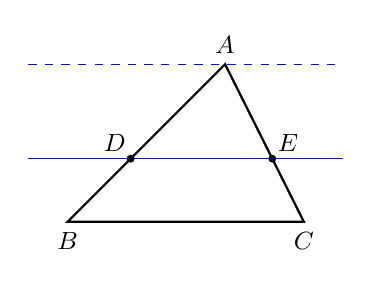
\begin{tikzpicture}[scale=1,font=\small]
\usetikzlibrary{calc}

\begin{scope}
\coordinate (a) at (0,2);
\coordinate (b) at (-2,0);
\coordinate (c) at (1,0);

\coordinate (t1) at (-2.5,0.8);
\coordinate (t2) at (1.5,0.8);
\coordinate (r1) at (-2.5,2);
\coordinate (r2) at (1.5,2);
\coordinate (d) at (intersection of t1--t2 and a--b);
\coordinate (e) at (intersection of t1--t2 and a--c);

\draw[thick] (a) node[above] {$A$} -- (b) node[below] {$B$} -- (c) node[below] {$C$} -- cycle;
\draw[blue] (t1) -- (t2);
\draw[dashed, blue] (r1) -- (r2);

\draw[fill] (d) circle (1.2pt) node[shift={(-0.2,0.2)}] {$D$};
\draw[fill] (e) circle (1.2pt) node[shift={(0.2,0.2)}] {$E$};

\end{scope}

\end{tikzpicture}
	
\end{figure*}

\begin{proof}
Sia $ABC$ il triangolo in questione. Tracciamo una retta parallela al 
lato $BC$ che intersechi gli altri due nei punti $D$ ed $E$. Vogliamo 
dimostrare che $AE : AD = EC : DB$.

Tracciamo una retta passante per $A$ e parallela a $DE$ ed a $BC$. Ci 
troviamo così nelle condizioni di poter applicare il teorema di 
Talete, in quanto abbiamo tre rette parallele tagliate da due 
trasversali ($AB$ ed $AC$), per cui possiamo scrivere la proporzione 
tra segmenti corrispondenti $AE : AD = EC : DB$.
La stessa dimostrazione vale nel caso in cui la parallela al lato 
$BC$ interseca i prolungamenti dei lati $AB$ e $AC$.
\end{proof}

\begin{corollario}\label{cor:6.2}
La retta che divide due lati di un triangolo (o i loro prolungamenti) 
in segmenti proporzionali è parallela al terzo lato.
\end{corollario}

\begin{figure*}[!htb]
	\centering% Copyright (c) 2015 Daniele Masini - d.masini.it@gmail.com

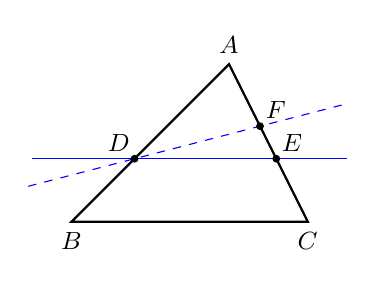
\begin{tikzpicture}[scale=1,font=\small]
\usetikzlibrary{calc}

\begin{scope}
\coordinate (a) at (0,2);
\coordinate (b) at (-2,0);
\coordinate (c) at (1,0);

\coordinate (t1) at (-2.5,0.8);
\coordinate (t2) at (1.5,0.8);
\coordinate (d) at (intersection of t1--t2 and a--b);
\coordinate (e) at (intersection of t1--t2 and a--c);
\coordinate (r1) at (d);
\coordinate (r2) at (1.5,1.5);

\draw[thick] (a) node[above] {$A$} -- (b) node[below] {$B$} -- (c) node[below] {$C$} -- cycle;
\draw[blue] (t1) -- (t2);
\draw[dashed, blue] ($(r1)!-.5!(r2)$) -- (r2);
\coordinate (f) at (intersection of r1--r2 and a--c);

\draw[fill] (d) circle (1.2pt) node[shift={(-0.2,0.2)}] {$D$};
\draw[fill] (e) circle (1.2pt) node[shift={(0.2,0.2)}] {$E$};
\draw[fill] (f) circle (1.2pt) node[shift={(0.2,0.2)}] {$F$};

\end{scope}

\end{tikzpicture}
	
\end{figure*}

\begin{proof}
Abbiamo in ipotesi che $AE : AD = AC : AB$ e dobbiamo dimostrare che 
$DE$ è parallela a $BC$.

Ragioniamo per assurdo; neghiamo quindi la tesi e supponiamo che DE 
non sia parallela a $BC$. Esisterà allora un'altra retta passante per 
$D$ parallela a $BC$; questa retta intersecherà il lato $AC$ in un 
punto $F$. Per il corollario~\ref{cor:6.1} avremo che $AF : AD = AC : 
AB$.
Ma per il teorema della quarta proporzionale sappiamo che la quarta 
grandezza che con le tre date forma una proporzione deve essere 
unica, e quindi il punto $F$ deve coincidere con $E$ e la retta $DF$ 
coincidere con la retta $DE$, che perciò è parallela a $BC$.
\end{proof}

Un'altra importante conseguenza del teorema di Talete è il 
\emph{teorema della bisettrice}.
\begin{teorema}[della bisettrice]
La bisettrice di un angolo interno di un triangolo divide il lato 
opposto in parti proporzionali agli altri due lati.
\end{teorema}

\noindent\begin{minipage}{0.65\textwidth}\parindent15pt
\noindent Ipotesi: $A\widehat{B}D\cong D\widehat{B}C$.\tab\tab Tesi: 
$AD : DC = AB : BC$.

\begin{proof}
Dal vertice $C$ tracciamo la parallela alla bisettrice $BD$ che 
incontra il prolungamento del lato $AB$ in $E$. Notiamo le seguenti 
congruenze tra angoli: $A\widehat{D}B\cong B\widehat{E}C$ in quanto 
corrispondenti rispetto alle parallele $BD$ ed $EC$ tagliate da $AE$; 
$D\widehat{B}C\cong B\widehat{C}E$ in quanto alterni interni rispetto 
alle parallele $BD$ ed $EC$ tagliate da $BC$.
Confrontando queste congruenze con quella in ipotesi ed applicando la 
proprietà transitiva della congruenza possiamo scrivere 
$B\widehat{E}C\cong B\widehat{C}E$. Dunque il triangolo $BEC$ è 
isoscele e per questo ha due lati congruenti $BE = BC$.
Applichiamo ora il primo corollario del teorema di Talete 
(corollario~\ref{cor:6.1}) al triangolo $AEC$. Si ha $AB : BE = AD : 
DC$. 
Per quanto appena dimostrato possiamo sostituire $BC$ a $BE$ ed 
avremo $AB : BC = AD : DC$.
\end{proof}
\end{minipage}\hfil
\begin{minipage}{0.35\textwidth}
	\centering% Copyright (c) 2015 Daniele Masini - d.masini.it@gmail.com

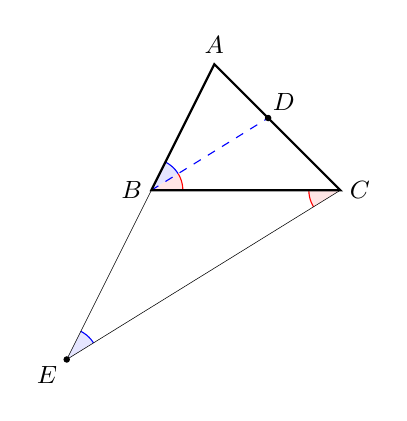
\begin{tikzpicture}[scale=0.8,font=\small]
\usetikzlibrary{calc}

\begin{scope}
\coordinate (a) at (-1,2);
\coordinate (b) at (-2,0);
\coordinate (c) at (1,0);

\path (b) let \p1 = ($(a)-(b)$) in -- ($(b)!{veclen(\x1,\y1)}!(c)$) -- +($(a)-(b)$) coordinate (ob);

\begin{scope}
\clip (a) -- (b) -- (ob) -- cycle;
\draw[blue, fill=blue!10] (b) circle (0.5);
\end{scope}

\begin{scope}
\clip (ob) -- (b) -- (c) -- cycle;
\draw[red, fill=red!10] (b) circle (0.5);
\end{scope}

\draw[blue, dashed] (b) -- (intersection of b--ob and a--c) coordinate (d);
\path (c) -- +($(b)-(d)$) coordinate (c1);
\coordinate (e) at (intersection of a--b and c--c1);

\begin{scope}
\clip (e) -- (c) -- (b) -- cycle;
\draw[red, fill=red!10] (c) circle (0.5);
\end{scope}

\begin{scope}
\clip (b) -- (e) -- (c) -- cycle;
\draw[blue, fill=blue!10] (e) circle (0.5);
\end{scope}

\draw[thick] (a) node[above] {$A$} -- (b) node[shift={(-0.25,0)}] {$B$} -- (c) node[shift={(0.25,0)}] {$C$} -- cycle;

\draw[very thin] (b) -- (e);
\draw[very thin] (c) -- (e);

\draw[fill] (d) circle (1.2pt) node[shift={(0.2,0.2)}] {$D$};
\draw[fill] (e) circle (1.2pt) node[shift={(-0.25,-0.2)}] {$E$};

\end{scope}

\end{tikzpicture}

\end{minipage}\vspace{5pt}

\subsubsection{Dividere un dato segmento in parti direttamente 
proporzionali a più segmenti dati}
\nopagebreak
\begin{wrapfigure}{r}{0.4\textwidth}
	\centering% Copyright (c) 2015 Daniele Masini - d.masini.it@gmail.com

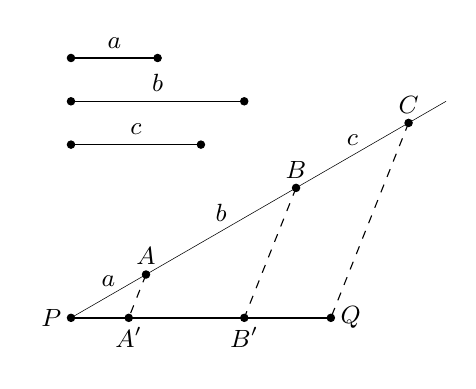
\begin{tikzpicture}[scale=1.1,font=\small]
\usetikzlibrary{calc}

\clip (-.5,-3.5) rectangle (4.35,0.35);

\begin{scope}
\coordinate (a1) at (0,0);
\coordinate (a2) at (1,0);
\coordinate (b1) at (0,-0.5);
\coordinate (b2) at (2,-0.5);
\coordinate (c1) at (0,-1);
\coordinate (c2) at (1.5,-1);
\draw (a1)-- node[above] {$a$} (a2);
\draw (b1)-- node[above] {$b$} (b2);
\draw (c1)-- node[above] {$c$} (c2);
\draw[fill] (a1) circle (1.2pt);
\draw[fill] (a2) circle (1.2pt);
\draw[fill] (b1) circle (1.2pt);
\draw[fill] (b2) circle (1.2pt);
\draw[fill] (c1) circle (1.2pt);
\draw[fill] (c2) circle (1.2pt);
\end{scope}

\begin{scope}[yshift=-3cm]
\coordinate (p) at (0,0);
\coordinate (p1) at (30:5);
\coordinate (a) at (30:1);
\coordinate (b) at (30:3);
\coordinate (c) at (30:4.5);
\coordinate (q) at (0:3);

\draw[very thin] (p)--(p1);
\draw[fill] (p) circle (1.2pt) node[left] {$P$};
\draw[fill] (a) circle (1.2pt) node[above] {$A$};
\draw[fill] (b) circle (1.2pt) node[above] {$B$};
\draw[fill] (c) circle (1.2pt) node[above] {$C$};

\draw[thick] (p)--(q);
\draw[dashed] (c)--(q);

\path (b) -- +($(q)-(c)$) coordinate (bx);
\path (a) -- +($(q)-(c)$) coordinate (ax);
\coordinate (b1) at (intersection of b--bx and p--q);
\coordinate (a1) at (intersection of a--ax and p--q);
\draw[dashed] (b) -- (b1);
\draw[dashed] (a) -- (a1);

\path (p) -- node[above] {$a$} (a);
\path (a) -- node[above] {$b$} (b);
\path (b) -- node[above] {$c$} (c);

\draw[fill] (a1) circle (1.2pt) node[below] {$A'$};
\draw[fill] (b1) circle (1.2pt) node[below] {$B'$};
\draw[fill] (q) circle (1.2pt) node[right] {$Q$};

\end{scope}

\end{tikzpicture}

\end{wrapfigure}
Sia $PQ$ il segmento da dividere in parti direttamente proporzionali 
a tre segmenti dati $a$, $b$ e $c$.
Da un suo estremo, ad esempio $P$, si tracci una semiretta (non 
contenente $Q$) e su di essa si prendano i segmenti $PA$, $AB$ e $BC$ 
rispettivamente congruenti ad $a$, $b$ e $c$; si unisca $C$ con $Q$ e 
si traccino per $A$ e per $B$ le parallele a $CQ$ che incontrano il 
segmento $PQ$ rispettivamente in $A'$ e $B'$. Il segmento $PQ$ 
risulta così diviso nei segmenti $PA'$, $A'B'$ e $B'Q$ che, per il 
teorema di Talete, sono direttamente proporzionali ai segmenti $a$, 
$b$ e $c$.

Da notare che se i segmenti dati fossero tutti fra loro congruenti, 
il problema equivarrebbe a quello della divisione di un dato segmento 
in un numero assegnato di parti congruenti.

\subsubsection{Costruire il segmento quarto proporzionale dopo tre 
segmenti dati}

\begin{wrapfigure}{r}{0.4\textwidth}
	\centering% Copyright (c) 2015 Daniele Masini - d.masini.it@gmail.com

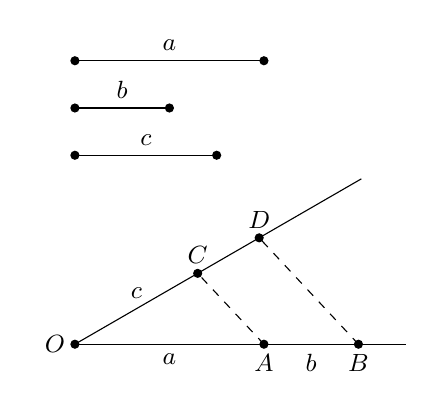
\begin{tikzpicture}[scale=1.2,font=\small]
\usetikzlibrary{calc}

\clip (-.5,-3.5) rectangle (3.55,0.35);

\begin{scope}
\coordinate (a1) at (0,0);
\coordinate (a2) at (2,0);
\coordinate (b1) at (0,-0.5);
\coordinate (b2) at (1,-0.5);
\coordinate (c1) at (0,-1);
\coordinate (c2) at (1.5,-1);
\draw (a1)-- node[above] {$a$} (a2);
\draw (b1)-- node[above] {$b$} (b2);
\draw (c1)-- node[above] {$c$} (c2);
\draw[fill] (a1) circle (1.2pt);
\draw[fill] (a2) circle (1.2pt);
\draw[fill] (b1) circle (1.2pt);
\draw[fill] (b2) circle (1.2pt);
\draw[fill] (c1) circle (1.2pt);
\draw[fill] (c2) circle (1.2pt);
\end{scope}

\begin{scope}[yshift=-3cm]
\coordinate (p) at (0,0);
\coordinate (p1) at (0:3.5);
\coordinate (p2) at (30:3.5);
\coordinate (a) at (0:2);
\coordinate (b) at (0:3);
\coordinate (c) at (30:1.5);
\path (b) -- +($(c)-(a)$) coordinate (bx);
\coordinate (d) at (intersection of b--bx and p--p2);

\draw (p)--(p1);
\draw (p)--(p2);

\path (p) -- node[below] {$a$} (a);
\path (p) -- node[above] {$c$} (c);
\path (a) -- node[below] {$b$} (b);

\draw[fill] (p) circle (1.2pt) node[left] {$O$};
\draw[fill] (a) circle (1.2pt) node[below] {$A$};
\draw[fill] (b) circle (1.2pt) node[below] {$B$};
\draw[fill] (c) circle (1.2pt) node[above] {$C$};
\draw[fill] (d) circle (1.2pt) node[above] {$D$};

\draw[dashed] (a)--(c);
\draw[dashed] (b)--(d);

\end{scope}

\end{tikzpicture}

\end{wrapfigure}
Siano $a$, $b$, $c$ i tre segmenti dati; si vuol costruire un 
segmento $d$ tale che valga la proporzione $a:b=c:d$.
Si consideri un angolo di vertice $O$ e su un suo lato si prendano i 
punti $A$ e $B$ tali che i segmenti $OA$ ed $AB$ siano congruenti 
rispettivamente ai segmenti $a$ e $b$; sull'altro lato dell'angolo si 
prenda il punto $C$ tale che il segmento $OC$ sia congruente al 
segmento $c$. Si traccino la retta $AC$ e la parallela ad essa per 
$B$, indicando con $D$ il punto in cui quest'ultima incontra la 
semiretta $OC$. Per il teorema di Talete il segmento $CD$ è il quarto 
proporzionale richiesto. 

Si noti che, per il teorema della quarta proporzionale, il segmento 
richiesto è unico, quindi si giunge allo stesso segmento 
indipendentemente dall'angolo utilizzato nella costruzione.

Nel caso particolare in cui $b = c$, la costruzione appena descritta 
consente di trovare il segmento terzo proporzionale a due segmenti 
dati.

\subsubsection{Proprietà}

\begin{wrapfigure}{r}{0.45\textwidth}
	\centering% Copyright (c) 2015 Daniele Masini - d.masini.it@gmail.com

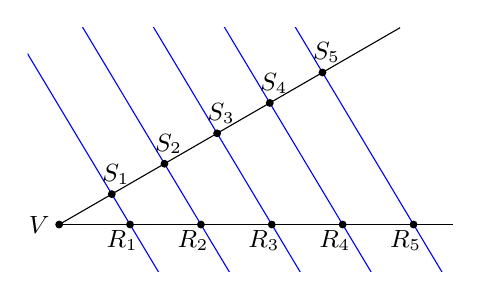
\begin{tikzpicture}[scale=1,font=\small]
\usetikzlibrary{calc}

\begin{scope}
\clip (-0.4,-0.6) rectangle (5,2.5);
\coordinate (v) at (0,0);
\coordinate (s) at (30:5);
\coordinate (r) at (0:5);
\coordinate (t11) at (1.5,-1);
\coordinate (t21) at (0,1.5);
\coordinate (S1) at (intersection of t11--t21 and v--s);
\coordinate (R1) at (intersection of t11--t21 and v--r);
\path (R1) let \p1 = ($(R1)-(v)$) in -- +($(v)!{veclen(\x1,\y1)}!(R1)$) coordinate (R2);
\path (R2) -- +($(S1)-(R1)$) coordinate (P2);
\coordinate (S2) at (intersection of R2--P2 and v--s);
\path (R1) let \p1 = ($(R2)-(R1)$) in -- +($(R1)!{veclen(\x1,\y1)}!(R2)$) coordinate (R3);
\path (R3) -- +($(S2)-(R2)$) coordinate (P3);
\coordinate (S3) at (intersection of R3--P3 and v--s);
\path (R1) let \p1 = ($(R3)-(R2)$) in -- +($(R2)!{veclen(\x1,\y1)}!(R3)$) coordinate (R4);
\path (R4) -- +($(S3)-(R3)$) coordinate (P4);
\coordinate (S4) at (intersection of R4--P4 and v--s);
\path (R1) let \p1 = ($(R4)-(R3)$) in -- +($(R3)!{veclen(\x1,\y1)}!(R4)$) coordinate (R5);
\path (R5) -- +($(S4)-(R4)$) coordinate (P5);
\coordinate (S5) at (intersection of R5--P5 and v--s);

\draw (v) -- (r);
\draw (v) -- (s);
\draw[blue] ($(R1)!-2!(S1)$) -- ($(R1)!6!(S1)$);
\draw[blue] ($(R2)!-2!(S2)$) -- ($(R2)!4!(S2)$);
\draw[blue] ($(R3)!-2!(S3)$) -- ($(R3)!4!(S3)$);
\draw[blue] ($(R4)!-2!(S4)$) -- ($(R4)!4!(S4)$);
\draw[blue] ($(R5)!-2!(S5)$) -- ($(R5)!4!(S5)$);
\draw[fill] (v) circle (1.2pt) node[left] {$V$};
\draw[fill] (S1) circle (1.2pt) node[shift={(0.05,0.25)}] {$S_1$};
\draw[fill] (R1) circle (1.2pt) node[shift={(-0.1,-0.2)}] {$R_1$};
\draw[fill] (S2) circle (1.2pt) node[shift={(0.05,0.25)}] {$S_2$};
\draw[fill] (R2) circle (1.2pt) node[shift={(-0.1,-0.2)}] {$R_2$};
\draw[fill] (S3) circle (1.2pt) node[shift={(0.05,0.25)}] {$S_3$};
\draw[fill] (R3) circle (1.2pt) node[shift={(-0.1,-0.2)}] {$R_3$};
\draw[fill] (S4) circle (1.2pt) node[shift={(0.05,0.25)}] {$S_4$};
\draw[fill] (R4) circle (1.2pt) node[shift={(-0.1,-0.2)}] {$R_4$};
\draw[fill] (S5) circle (1.2pt) node[shift={(0.05,0.25)}] {$S_5$};
\draw[fill] (R5) circle (1.2pt) node[shift={(-0.1,-0.2)}] {$R_5$};

\end{scope}

\end{tikzpicture}

\end{wrapfigure}
Dato un angolo di vertice $V$ e lati due semirette $r$ ed $s$, 
staccare su $r$ il segmento $VR_5$ e su $s$ il segmento $VS_1$, di 
lunghezza arbitraria. Successivamente, usando un compasso, staccare 
su $s$ i segmenti $S_1S_2$, $S_2S_3$, $S_3S_4$ e $S_4S_5$, tutti 
congruenti a $VS_1$. Dimostrare che, tracciando la retta per $R_5S_5$ 
e le corrispondenti parallele per $S_1$, $S_2$, $S_3$ ed $S_4$, il 
segmento $VR_5$ risulta suddiviso in parti uguali.

Osservando che questo procedimento può essere esteso per induzione a 
qualunque numero finito di segmenti, si può constatare che la 
divisibilità di un segmento in parti uguali non è un postulato 
autonomo, ma una proprietà intrinseca della geometria euclidea.


\section{Avere la stessa forma}\label{sect:stessa_forma}

\begin{wrapfigure}{r}{0.37\textwidth}
	\centering% Copyright (c) 2015 Daniele Masini - d.masini.it@gmail.com

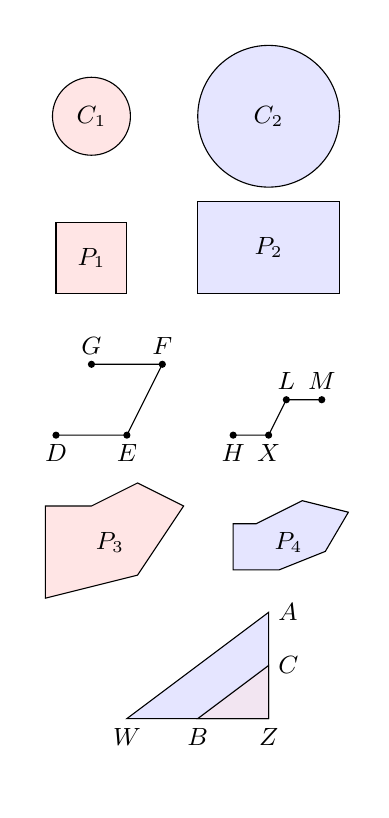
\begin{tikzpicture}[scale=.9,font=\small]
\usetikzlibrary{calc}

\clip (-0.9,-9.5) rectangle (3.8,1.25);

\begin{scope}
\coordinate (o1) at (0,0);
\coordinate (o2) at (2.5,0);

\draw[fill=red!10] (o1) circle(0.55);
\draw[fill=blue!10] (o2) circle(1);
%\draw[fill] (o1) circle (1.2pt) node[left] {$O_1$};
%\draw[fill] (o2) circle (1.2pt) node[left] {$O_2$};
\node at (o1) {$C_1$};
\node at (o2) {$C_2$};

\end{scope}


\begin{scope}[yshift=-2.5cm, xshift=-.5cm]
\draw[fill=red!10] (0,0) rectangle (1,1);
\draw[fill=blue!10] (2,0) rectangle (4,1.3);
\node at (0.5,0.5) {$P_1$};
\node at (3,0.65) {$P_2$};

\end{scope}


\begin{scope}[yshift=-3.5cm, xshift=0cm]
\coordinate (g) at (0,0);
\coordinate (f) at (1,0);
\coordinate (e) at (0.5,-1);
\coordinate (d) at (-0.5,-1);
\coordinate (h) at (2,-1);
\coordinate (x) at (2.5,-1);
\coordinate (l) at (2.75,-0.5);
\coordinate (m) at (3.25,-0.5);

\draw (g) -- (f) -- (e) -- (d);
\draw[fill] (g) circle (1.2pt) node[above] {$G$};
\draw[fill] (f) circle (1.2pt) node[above] {$F$};
\draw[fill] (e) circle (1.2pt) node[below] {$E$};
\draw[fill] (d) circle (1.2pt) node[below] {$D$};
\draw (h) -- (x) -- (l) -- (m);
\draw[fill] (h) circle (1.2pt) node[below] {$H$};
\draw[fill] (x) circle (1.2pt) node[below] {$X$};
\draw[fill] (l) circle (1.2pt) node[above] {$L$};
\draw[fill] (m) circle (1.2pt) node[above] {$M$};

\end{scope}


\begin{scope}[yshift=-5.5cm]
\begin{scope}[scale=1.3, xshift=-0.5cm]
\coordinate (p1) at (0,0);
\coordinate (p2) at (0.5,0);
\coordinate (p3) at (1,0.25);
\coordinate (p4) at (1.5,0);
\coordinate (p5) at (1,-0.75);
\coordinate (p6) at (0,-1);
\draw[fill=red!10] (p1) -- (p2) -- (p3) -- (p4) -- (p5) -- (p6) -- cycle;
\node at (0.7,-0.4) {$P_3$};
\end{scope}
\begin{scope}[yshift=-.25cm, xshift=2cm, scale=1.3]
\coordinate (q1) at (0,0);
\coordinate (q2) at (0.25,0);
\coordinate (q3) at (0.75,0.25);
\coordinate (q4) at (1.25,0.125);
\coordinate (q5) at (1,-0.30);
\coordinate (q6) at (0.5,-0.5);
\coordinate (q7) at (0,-0.5);
\draw[fill=blue!10] (q1) -- (q2) -- (q3) -- (q4) -- (q5) -- (q6) -- (q7) -- cycle;
\node at (0.6,-0.2) {$P_4$};
\end{scope}

\end{scope}


\begin{scope}[yshift=-7cm, xshift=2.5cm]
\coordinate (a) at (0,0);
\coordinate (b) at (-1,-1.5);
\coordinate (c) at (0,-0.75);
\coordinate (w) at (-2,-1.5);
\coordinate (z) at (0,-1.5);

\draw[fill=blue!10] (a) node[right] {$A$} -- (z) node[below] {$Z$} -- (w) node[below] {$W$} -- cycle;
\path[fill=red!10, opacity=.5] (b) -- (c) -- (z) -- cycle;
\draw (b) node[below] {$B$} -- (c) node[right] {$C$} -- (z) -- cycle;

\end{scope}



\end{tikzpicture}

\end{wrapfigure}
Osserviamo le coppie di figure rappresentate a lato e cerchiamo di 
capire cosa intendiamo dire quando affermiamo che due figure hanno  
la stessa forma.

I due cerchi $C_1$ e $C_1$ hanno certamente la stessa forma.

I poligoni $P_1$ e $P_2$ hanno gli angoli rispettivamente congruenti, 
ma non possiamo dire che abbiano la stessa forma.

I segmenti di $HKLM$ sono rispettivamente la metà dei segmenti di 
$DEFG$, ma anche in questo caso non possiamo dire che i due disegni 
abbiano la stessa forma: gli angoli formati dai segmenti non sono 
rispettivamente congruenti.

I poligoni $P_3$ e $P_4$ non hanno la stessa forma, addirittura non 
hanno lo stesso numero di lati.

I triangoli $AWZ$ e $BCZ$ hanno la stessa forma. Hanno gli angoli 
rispettivamente congruenti. Inoltre, essendo $B$ punto medio di $WZ$ 
e $C$ punto medio di $AZ$, i lati di $BCZ$ sono ciascuno la metà dei 
corrispondenti lati del triangolo $AWZ$, anche il lato $BC$ che 
congiunge i punti è la metà di $AW$, per un teorema che hai già 
studiato; in definitiva, il rapporto tra $BC$ e $WA$, tra $BZ$ e 
$WZ$, tra $CZ$ e $AZ$ è sempre di 1 a 2; i lati sono quindi in 
proporzione  $AZ : CZ = WZ : BZ = AW : BC$.

\begin{definizione}
Due poligoni $P$ e $Q$ aventi angoli rispettivamente congruenti e 
lati in proporzione si dicono \emph{simili} e scriviamo $P\sim Q$.
\end{definizione}

\begin{wrapfigure}{r}{0.55\textwidth}
	\centering% Copyright (c) 2015 Daniele Masini - d.masini.it@gmail.com

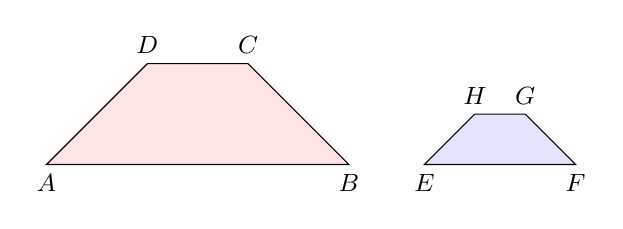
\begin{tikzpicture}[scale=.8,font=\small]
\usetikzlibrary{calc}

\begin{scope}[scale=0.8]
\coordinate (a) at (0,0);
\coordinate (b) at (6,0);
\coordinate (c) at (4,2);
\coordinate (d) at (2,2);

\draw[fill=red!10] (a) node[below] {$A$} -- (b) node[below] {$B$} -- (c) node[above] {$C$} -- (d) node[above] {$D$} -- cycle;

\end{scope}


\begin{scope}[xshift=6cm, scale=0.4]
\coordinate (a) at (0,0);
\coordinate (b) at (6,0);
\coordinate (c) at (4,2);
\coordinate (d) at (2,2);

\draw[fill=blue!10] (a) node[below] {$E$} -- (b) node[below] {$F$} -- (c) node[above] {$G$} -- (d) node[above] {$H$} -- cycle;
\end{scope}

\end{tikzpicture}

\end{wrapfigure}
Nella figura precedente, i due triangoli $AWZ$ e $CBZ$ sono simili.
Sono simili anche i due trapezi della figura a lato, hanno infatti 
gli angoli congruenti e i lati in proporzione: i lati del primo 
trapezio sono tutti il doppio di quelli del secondo trapezio.

\begin{definizione}
Si chiamano \emph{omologhi} sia i vertici degli angoli 
rispettivamente congruenti sia i lati e le diagonali che congiungono 
vertici omologhi. Si chiama \emph{rapporto di similitudine} il 
rapporto tra due lati omologhi.
\end{definizione}

Relativamente ai due trapezi della figura precedente:
\begin{itemize*}
\item sono vertici omologhi $A$ ed $E$; \ldots{} e \ldots{}; \ldots{} 
e \ldots{}; \ldots{} e \ldots{};
\item sono lati omologhi $DC$ e $HG$; \ldots\ldots{} e 
\ldots\ldots{}; \ldots\ldots{} e \ldots\ldots{}; \ldots\ldots{} e 
\ldots\ldots{};
\item sono diagonali omologhe \ldots\ldots{} e \ldots\ldots{}; 
\ldots\ldots{} e \ldots\ldots{};
\item il rapporto di similitudine è \ldots\ldots{}
\end{itemize*}

\osservazione Se due poligoni sono congruenti allora sono anche 
simili con rapporto di similitudine 1.


\section{La similitudine nei 
triangoli}\label{sect:similitudine_triangoli}

La definizione di triangoli simili non si differenzia da quella data 
per i poligoni. Per i triangoli, però, esistono dei teoremi, detti 
criteri, che permettono di verificare se due triangoli sono simili 
restringendo le verifiche da  effettuare.

\begin{teorema}[1\textsuperscript{o} criterio di similitudine]
Due triangoli aventi due angoli rispettivamente congruenti sono 
simili.
\end{teorema}

\begin{figure*}[!htb]
	\centering% Copyright (c) 2015 Daniele Masini - d.masini.it@gmail.com

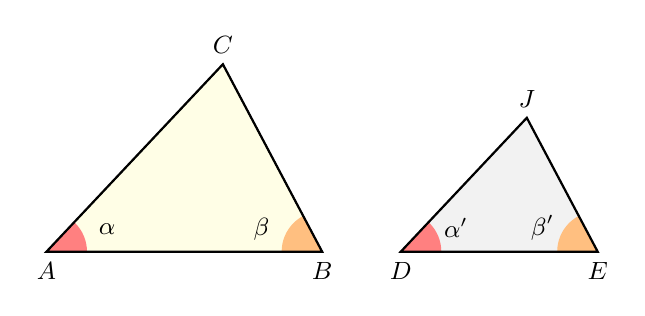
\begin{tikzpicture}[scale=1,font=\small]
\usetikzlibrary{calc}

\begin{scope}[scale=1.4]
\coordinate (a) at (0,0);
\coordinate (c) at (1.6,1.7);
\coordinate (b) at (2.5,0);
\draw[fill=yellow!10] (a) -- (b) -- (c) -- cycle;

\begin{scope}
\clip (a) -- (b) -- (c) -- cycle;
\draw[thick,red!50,fill] (a) circle ({0.5*0.714285714});
\node at ([shift={(0.55,0.2)}]a) {$\alpha$};
\draw[thick,orange!50,fill] (b) circle ({0.5*0.714285714});
\node at ([shift={(-0.55,0.2)}]b) {$\beta$};
\end{scope}

\draw[thick] (a) node[below] {$A$} -- (b) node[below] {$B$} -- (c) node[above] {$C$} -- cycle;


\end{scope}

\begin{scope}[xshift=4.5cm, scale=1]
\coordinate (a) at (0,0);
\coordinate (c) at (1.6,1.7);
\coordinate (b) at (2.5,0);
\draw[fill=gray!10] (a) -- (b) -- (c) -- cycle;

\begin{scope}
\clip (a) -- (b) -- (c) -- cycle;
\draw[thick,red!50,fill] (a) circle (0.5);
\node at ([shift={(0.7,0.3)}]a) {$\alpha'$};
\draw[thick,orange!50,fill] (b) circle (0.5);
\node at ([shift={(-0.7,0.3)}]b) {$\beta'$};
\end{scope}

\draw[thick] (a) node[below] {$D$} -- (b) node[below] {$E$} -- (c) node[above] {$J$} -- cycle;

\end{scope}

\end{tikzpicture}
\hspace{2cm}% Copyright (c) 2015 Daniele Masini - d.masini.it@gmail.com

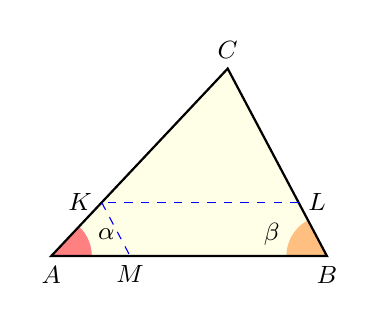
\begin{tikzpicture}[scale=1,font=\small]
\usetikzlibrary{calc}

\clip (-0.3,-0.4) rectangle (3.8,2.9);

\begin{scope}[scale=1.4]
\coordinate (a) at (0,0);
\coordinate (c) at (1.6,1.7);
\coordinate (b) at (2.5,0);
\draw[fill=yellow!10] (a) -- (b) -- (c) -- cycle;

\begin{scope}
\clip (a) -- (b) -- (c) -- cycle;
\draw[thick,red!50,fill] (a) circle ({0.5*0.714285714});
\node at ([shift={(0.50,0.2)}]a) {$\alpha$};
\draw[thick,orange!50,fill] (b) circle ({0.5*0.714285714});
\node at ([shift={(-0.50,0.2)}]b) {$\beta$};
\end{scope}

\draw[thick] (a) node[below] {$A$} -- (b) node[below] {$B$} -- (c) node[above] {$C$} -- cycle;
\draw[blue, dashed] ($(c)!0.714285714!(b)$) coordinate (l) node[black, right] {$L$} -- ($(c)!0.714285714!(a)$) coordinate (k) node[black, left] {$K$};
\path (k) -- +($(b)-(c)$) coordinate (k1);
\coordinate (m) at (intersection of k--k1 and a--b);
\draw[blue, dashed] (k) -- (m) node [black, below] {$M$};
%\draw[fill] (k) circle (1pt);
%\draw[fill] (m) circle (1pt);
%\draw[fill] (l) circle (1pt);

\end{scope}

\end{tikzpicture}

\end{figure*}

\begin{proof}
Osserviamo che se due triangoli hanno due angoli congruenti, per il 
teorema della somma degli angoli interni di un triangolo, avranno 
anche il terzo angolo congruente.
Nella figura, i due triangoli $ABC$ e $DEJ$ hanno $\widehat{A}\cong 
\widehat{D}$ e $\widehat{B}\cong \widehat{E}$ di conseguenza 
$\widehat{C}\cong \widehat{J}$. Vogliamo dimostrare che i due 
triangoli hanno anche i lati in proporzione.

Se $DJ=AC$ i due triangoli sarebbero congruenti per il secondo 
criterio di congruenza, in quanto hanno un lato e i due angoli 
adiacenti rispettivamente congruenti, dunque anche simili, il 
rapporto di similitudine sarebbe 1.
Esaminiamo allora il caso $DJ\neq AC$, in particolare $DJ<AC$. Su 
$AC$ fissiamo un punto $K$ in modo che $CK=DJ$ e tracciamo da questo 
la parallela al lato $AB$ che incontra $CB$ in $L$; il triangolo 
$CKL$ risulta congruente al triangolo $DJE$ avendo $CK\cong DJ$, 
$\widehat{K}\cong \widehat{D}$ e $\widehat{C}\cong \widehat{J}$.
Inoltre per il teorema di Talete possiamo scrivere la proporzione $CA 
: CK = CB : CL$. Se tracciamo da $K$ la parallela al lato $CB$ che 
incontra $AB$ in $M$, per il teorema di Talete si ha $CA : CK = AB : 
MB$.
Per costruzione $KLBM$ è un parallelogramma, quindi $KL=MB$ e 
sostituendolo nella precedente proporzione otteniamo $CA : CK = AB : 
KL$. 
Confrontando le proporzioni ottenute possiamo scrivere $CA : CK = AB 
: KL = CB : CL$ e dalla congruenza tra i triangoli $CKL$ e $DJE$ 
concludiamo che $CA : DJ = AB : DE = CB : JE$.
\end{proof}


\begin{teorema}[2\textsuperscript{o} criterio di similitudine]
Due triangoli aventi due lati in proporzione e l'angolo tra essi 
compreso congruente sono simili.
\end{teorema}

%Con riferimento alla figura
\noindent Ipotesi: $AC : DF = AB : DE$, $\widehat{A}\cong 
\widehat{D}$.\tab Tesi: $B\cong E$, $C\cong F$, $CB : FE = AB : DE$.

\begin{figure*}[!htb]
	\centering% Copyright (c) 2015 Daniele Masini - d.masini.it@gmail.com

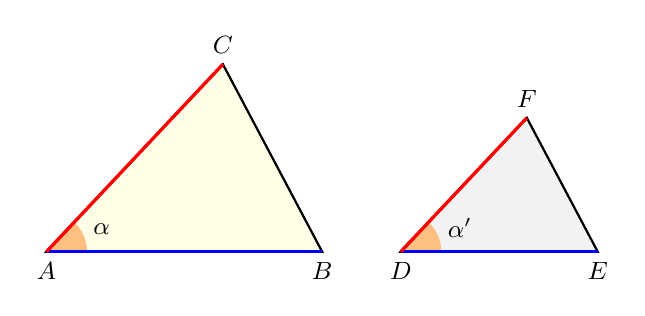
\begin{tikzpicture}[scale=1,font=\small]
\usetikzlibrary{calc}

\begin{scope}[scale=1.4]
\coordinate (a) at (0,0);
\coordinate (c) at (1.6,1.7);
\coordinate (b) at (2.5,0);
\draw[fill=yellow!10] (a) -- (b) -- (c) -- cycle;

\begin{scope}
\clip (a) -- (b) -- (c) -- cycle;
\draw[thick,orange!50,fill] (a) circle ({0.5*0.714285714});
\node at ([shift={(0.5,0.2)}]a) {$\alpha$};
\end{scope}

\draw[thick] (a) node[below] {$A$} -- (b) node[below] {$B$} -- (c) node[above] {$C$} -- cycle;
\draw[blue,very thick] (a) -- (b);
\draw[red,very thick] (a) -- (c);

\end{scope}

\begin{scope}[xshift=4.5cm, scale=1]
\coordinate (a) at (0,0);
\coordinate (c) at (1.6,1.7);
\coordinate (b) at (2.5,0);
\draw[fill=gray!10] (a) -- (b) -- (c) -- cycle;

\begin{scope}
\clip (a) -- (b) -- (c) -- cycle;
\draw[thick,orange!50,fill] (a) circle (0.5);
\node at ([shift={(0.75,0.3)}]a) {$\alpha'$};
\end{scope}

\draw[thick] (a) node[below] {$D$} -- (b) node[below] {$E$} -- (c) node[above] {$F$} -- cycle;
\draw[blue,very thick] (a) -- (b);
\draw[red,very thick] (a) -- (c);

\end{scope}


\end{tikzpicture}
\hspace{2cm}% Copyright (c) 2015 Daniele Masini - d.masini.it@gmail.com

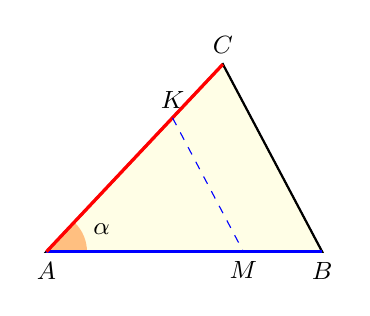
\begin{tikzpicture}[scale=1,font=\small]
\usetikzlibrary{calc}

\begin{scope}[scale=1.4]
\coordinate (a) at (0,0);
\coordinate (c) at (1.6,1.7);
\coordinate (b) at (2.5,0);
\draw[fill=yellow!10] (a) -- (b) -- (c) -- cycle;

\begin{scope}
\clip (a) -- (b) -- (c) -- cycle;
\draw[thick,orange!50,fill] (a) circle ({0.5*0.714285714});
\node at ([shift={(0.5,0.2)}]a) {$\alpha$};
\end{scope}

\draw[thick] (a) node[below] {$A$} -- (b) node[below] {$B$} -- (c) node[above] {$C$} -- cycle;
\draw[blue,very thick] (a) -- (b);
\draw[red,very thick] (a) -- (c);

\coordinate (k) at ($(a)!0.714285714!(c)$);
\coordinate (m) at ($(a)!0.714285714!(b)$);
\draw[blue, dashed] (k) node[black, above] {$K$} -- (m) node[black, below] {$M$};
%\draw[fill] (k) circle (1pt);
%\draw[fill] (m) circle (1pt);

\end{scope}


\end{tikzpicture}

\end{figure*}

\begin{proof}
Se $DF=AC$, dalla proporzione in ipotesi $AC:DF=AB:DE$ si avrebbe 
$DE\cong AB$ e i due triangoli sarebbero congruenti per il primo 
criterio di congruenza, pertanto anche simili.
Supponiamo $AC>DF$; su $AC$ fissiamo un punto $K$ in modo che 
$AK=DF$, da $K$ tracciamo la parallela a $CB$ che incontra $AB$ in 
$M$. Si ha che $\widehat{M}\cong \widehat{B}$ e $\widehat{K}\cong 
\widehat{C}$ perché corrispondenti delle rette parallele $KM$ e $CB$ 
rispettivamente con trasversale $AB$ e $AC$, dunque $AMK$ e $ABC$ 
sono simili per il primo criterio di similitudine, quindi 
$AB:AM=AC:AK=CB:KM$.

Confrontiamo i primi due rapporti con l'ipotesi. $AK=DF$ per 
costruzione, quindi $AM=DE$ poiché la grandezza quarta proporzionale 
dopo tre date è unica.
I due triangoli $AKM$ e $DFE$ risultano congruenti avendo $AK=DF$ per 
costruzione, $AM=DE$ per averlo dimostrato, $\widehat{A}\cong 
\widehat{D}$. Di conseguenza i due triangoli hanno anche gli altri 
elementi congruenti, cioè $KM=DE$, $\widehat{M}\cong \widehat{E}$ e 
$\widehat{K}\cong \widehat{F}$. Dai risultati ottenuti possiamo 
concludere che $AB:DE=AC:DF=BC:FE$.
\end{proof}

\begin{teorema}[3\textsuperscript{o} criterio di similitudine]
Due triangoli aventi i lati in proporzione sono simili.
\end{teorema}

\noindent Ipotesi: $AC : DF = AB : DE = CB : EF$.\tab Tesi: 
$\widehat{A}\cong \widehat{D}$, $\widehat{B}\cong \widehat{E}$, 
$\widehat{C}\cong \widehat{F}$.

\begin{figure*}[!htb]
	\centering% Copyright (c) 2015 Daniele Masini - d.masini.it@gmail.com

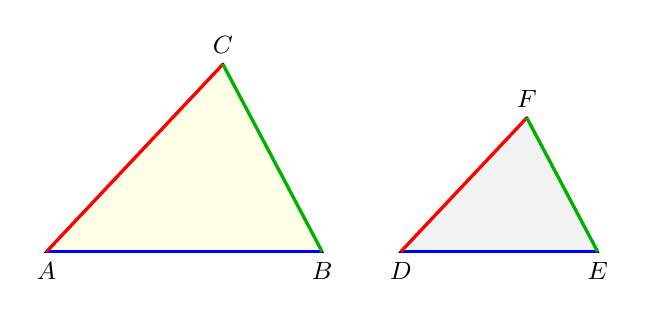
\begin{tikzpicture}[scale=1,font=\small]
\usetikzlibrary{calc}

\begin{scope}[scale=1.4]
\coordinate (a) at (0,0);
\coordinate (c) at (1.6,1.7);
\coordinate (b) at (2.5,0);
\draw[fill=yellow!10] (a) -- (b) -- (c) -- cycle;

\draw[thick] (a) node[below] {$A$} -- (b) node[below] {$B$} -- (c) node[above] {$C$} -- cycle;
\draw[blue,very thick] (a) -- (b);
\draw[red,very thick] (a) -- (c);
\draw[green!70!black,very thick] (b) -- (c);

\end{scope}

\begin{scope}[xshift=4.5cm, scale=1]
\coordinate (a) at (0,0);
\coordinate (c) at (1.6,1.7);
\coordinate (b) at (2.5,0);
\draw[fill=gray!10] (a) -- (b) -- (c) -- cycle;

\draw[thick] (a) node[below] {$D$} -- (b) node[below] {$E$} -- (c) node[above] {$F$} -- cycle;
\draw[blue,very thick] (a) -- (b);
\draw[red,very thick] (a) -- (c);
\draw[green!70!black,very thick] (b) -- (c);

\end{scope}


\end{tikzpicture}
\hspace{2cm}% Copyright (c) 2015 Daniele Masini - d.masini.it@gmail.com

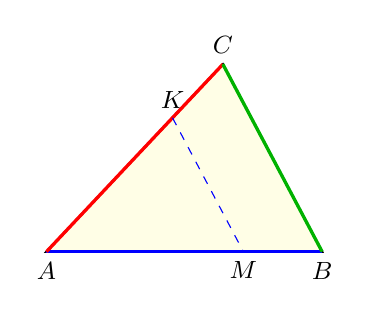
\begin{tikzpicture}[scale=1,font=\small]
\usetikzlibrary{calc}

\begin{scope}[scale=1.4]
\coordinate (a) at (0,0);
\coordinate (c) at (1.6,1.7);
\coordinate (b) at (2.5,0);
\draw[fill=yellow!10] (a) -- (b) -- (c) -- cycle;

\draw[thick] (a) node[below] {$A$} -- (b) node[below] {$B$} -- (c) node[above] {$C$} -- cycle;
\draw[blue,very thick] (a) -- (b);
\draw[red,very thick] (a) -- (c);
\draw[green!70!black,very thick] (b) -- (c);

\coordinate (k) at ($(a)!0.714285714!(c)$);
\coordinate (m) at ($(a)!0.714285714!(b)$);
\draw[blue, dashed] (k) node[black, above] {$K$} -- (m) node[black, below] {$M$};
%\draw[fill] (k) circle (1pt);
%\draw[fill] (m) circle (1pt);

\end{scope}


\end{tikzpicture}

\end{figure*}

\begin{proof}
Se $DF=AC$, dall'ipotesi si avrebbe anche $DE=AB$ e $FE=CB$, i due 
triangoli sarebbero allora congruenti per il terzo criterio di 
congruenza e dunque anche simili.
Supponiamo $AC>DF$; su $AC$ fissiamo un punto $K$ in modo che $AK=DF$ 
e da questo tracciamo la parallela a $CB$ che incontra $AB$ in $M$ 
ottenendo $\widehat{M}\cong \widehat{B}$ e $\widehat{K}\cong 
\widehat{C}$ perché corrispondenti delle rette parallele $KM$ e $CB$ 
rispettivamente con trasversale $AB$ e $AC$. Per il 
1\textsuperscript{o} criterio di similitudine $ABC\sim AKM$, possiamo 
allora scrivere $AC:AK=AB:AM=CB:KM$; confrontandola con la 
proporzione nell'ipotesi e tenendo presente la costruzione effettuata 
e l'unicità della quarta proporzionale, si deducono le congruenze 
$AM=DE$ e $KM=EF$. Pertanto risulta $AMK\cong DEF$ per il 
3\textsuperscript{o} criterio di congruenza e dunque anche 
$\widehat{A}\cong \widehat{D}$, $\widehat{M}\cong \widehat{E}$, 
$\widehat{K}\cong \widehat{F}$; quindi anche $\widehat{A}\cong 
\widehat{D}$, $\widehat{B}\cong \widehat{E}$, $\widehat{C}\cong 
\widehat{F}$.
\end{proof}

\subsection{Proprietà dei triangoli simili}

Nei paragrafi precedenti abbiamo dimostrato che in due triangoli 
simili, il rapporto tra due lati omologhi è uguale
\begin{itemize*}
\noindent\begin{minipage}{0.35\textwidth}\parindent15pt
\item al rapporto tra le rispettive altezze;
\end{minipage}\hfil
\begin{minipage}{0.65\textwidth}
	\centering% Copyright (c) 2015 Daniele Masini - d.masini.it@gmail.com

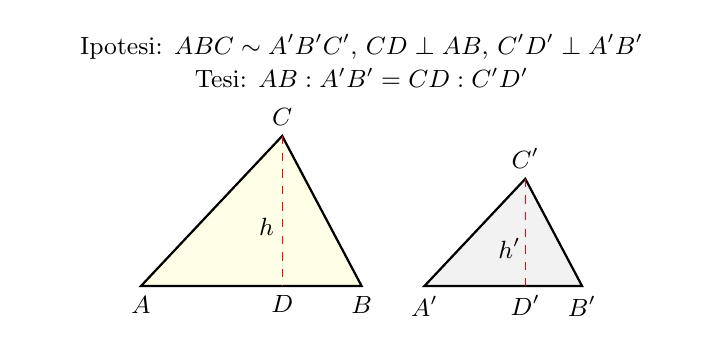
\begin{tikzpicture}[scale=0.8,font=\small]
\usetikzlibrary{calc}

\clip (-1.8,-0.7) rectangle (8.8,4.1);
\node at (3.5, 3.8) {Ipotesi: $ABC\sim A'B'C'$, $CD\perp AB$, $C'D'\perp A'B'$};
\node at (3.5, 3.3) {Tesi: $AB:A'B'=CD:C'D'$};

\begin{scope}[scale=1.4]
\coordinate (a) at (0,0);
\coordinate (c) at (1.6,1.7);
\coordinate (b) at (2.5,0);
\draw[fill=yellow!10] (a) -- (b) -- (c) -- cycle;

\draw[thick] (a) node[below] {$A$} -- (b) node[below] {$B$} -- (c) node[above] {$C$} -- cycle;
\draw[red, dashed] (c) -- node[black, shift={(-0.2,-0.2)}] {$h$} ($(a)!(c)!(b)$) node[black, below] {$D$};

\end{scope}

\begin{scope}[xshift=4.5cm, scale=1]
\coordinate (a) at (0,0);
\coordinate (c) at (1.6,1.7);
\coordinate (b) at (2.5,0);
\draw[fill=gray!10] (a) -- (b) -- (c) -- cycle;

\draw[thick] (a) node[below] {$A'$} -- (b) node[below] {$B'$} -- (c) node[above] {$C'$} -- cycle;
\draw[red, dashed] (c) -- node[black, shift={(-0.2,-0.2)}] {$h'$} ($(a)!(c)!(b)$) node[black, below] {$D'$};

\end{scope}


\end{tikzpicture}

\end{minipage}\vspace{5pt}
\noindent\begin{minipage}{0.35\textwidth}\parindent15pt
\item al rapporto tra le rispettive mediane;
\end{minipage}\hfil
\begin{minipage}{0.65\textwidth}
	\centering% Copyright (c) 2015 Daniele Masini - d.masini.it@gmail.com

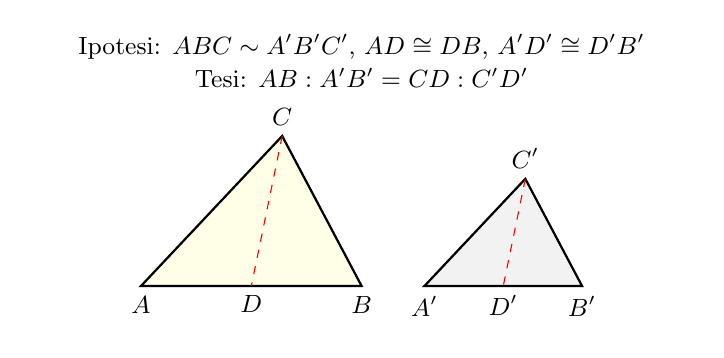
\begin{tikzpicture}[scale=0.8,font=\small]
\usetikzlibrary{calc}

\clip (-1.8,-0.7) rectangle (8.8,4.1);
\node at (3.5, 3.8) {Ipotesi: $ABC\sim A'B'C'$, $AD\cong DB$, $A'D'\cong D'B'$};
\node at (3.5, 3.3) {Tesi: $AB:A'B'=CD:C'D'$};

\begin{scope}[scale=1.4]
\coordinate (a) at (0,0);
\coordinate (c) at (1.6,1.7);
\coordinate (b) at (2.5,0);
\draw[fill=yellow!10] (a) -- (b) -- (c) -- cycle;

\draw[thick] (a) node[below] {$A$} -- (b) node[below] {$B$} -- (c) node[above] {$C$} -- cycle;
\draw[red, dashed] (c) -- ($(a)!0.5!(b)$) node[black, below] {$D$};

\end{scope}

\begin{scope}[xshift=4.5cm, scale=1]
\coordinate (a) at (0,0);
\coordinate (c) at (1.6,1.7);
\coordinate (b) at (2.5,0);
\draw[fill=gray!10] (a) -- (b) -- (c) -- cycle;

\draw[thick] (a) node[below] {$A'$} -- (b) node[below] {$B'$} -- (c) node[above] {$C'$} -- cycle;
\draw[red, dashed] (c) -- ($(a)!0.5!(b)$) node[black, below] {$D'$};

\end{scope}


\end{tikzpicture}

\end{minipage}\vspace{5pt}
\noindent\begin{minipage}{0.35\textwidth}\parindent15pt
\item al rapporto tra le bisettrici uscenti da due vertici omologhi.
\end{minipage}\hfil
\begin{minipage}{0.65\textwidth}
	\centering% Copyright (c) 2015 Daniele Masini - d.masini.it@gmail.com

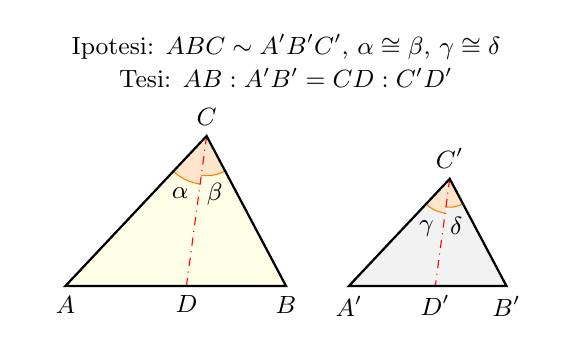
\begin{tikzpicture}[scale=0.8,font=\small]
\usetikzlibrary{calc}

\clip (-0.6,-0.65) rectangle (7.6,4.1);
\node at (3.5, 3.8) {Ipotesi: $ABC\sim A'B'C'$, $\alpha\cong\beta$, $\gamma\cong\delta$};
\node at (3.5, 3.3) {Tesi: $AB:A'B'=CD:C'D'$};

\begin{scope}[scale=1.4]
\coordinate (a) at (0,0);
\coordinate (c) at (1.6,1.7);
\coordinate (b) at (2.5,0);
\draw[fill=yellow!10] (a) -- (b) -- (c) -- cycle;

\path (c) let \p1 = ($(b)-(c)$) in -- ($(c)!{veclen(\x1,\y1)}!(a)$) -- +($(b)-(c)$) coordinate (c1);
\coordinate (d) at (intersection of c--c1 and a--b);

\begin{scope}
\clip (c) -- (a) -- (d) -- cycle;
\draw[orange, fill=orange!20] (c) circle (0.55) node[black, shift={(245:0.8)}] {$\alpha$};
\end{scope}

\begin{scope}
\clip (c) -- (d) -- (b) -- cycle;
\draw[orange, fill=orange!20] (c) circle (0.45) node[black, shift={(278:0.75)}] {$\beta$};
\end{scope}


\draw[red, dashdotted] (c) -- (d) node[black, below] {$D$};
\draw[thick] (a) node[below] {$A$} -- (b) node[below] {$B$} -- (c) node[above] {$C$} -- cycle;

\end{scope}

\begin{scope}[xshift=4.5cm, scale=1]
\coordinate (a) at (0,0);
\coordinate (c) at (1.6,1.7);
\coordinate (b) at (2.5,0);
\draw[fill=gray!10] (a) -- (b) -- (c) -- cycle;

\path (c) let \p1 = ($(b)-(c)$) in -- ($(c)!{veclen(\x1,\y1)}!(a)$) -- +($(b)-(c)$) coordinate (c1);
\coordinate (d) at (intersection of c--c1 and a--b);

\begin{scope}
\clip (c) -- (a) -- (d) -- cycle;
\draw[orange, fill=orange!20] (c) circle (0.55) node[black, shift={(245:0.7)}] {$\gamma$};
\end{scope}

\begin{scope}
\clip (c) -- (d) -- (b) -- cycle;
\draw[orange, fill=orange!20] (c) circle (0.45) node[black, shift={(278:0.6)}] {$\delta$};
\end{scope}

\draw[red, dashdotted] (c) -- (d) node[black, below] {$D'$};
\draw[thick] (a) node[below] {$A'$} -- (b) node[below] {$B'$} -- (c) node[above] {$C'$} -- cycle;

\end{scope}


\end{tikzpicture}

\end{minipage}\vspace{5pt}
\end{itemize*}

Ricordiamo che il rapporto di similitudine è il rapporto tra due lati 
omologhi.

\begin{teorema}\label{teo:6.3}% teorema 1
Il rapporto tra i perimetri di due triangoli simili è uguale al 
rapporto di similitudine.
\end{teorema}

\noindent Ipotesi: $AB:A'B'=AC:A'C'=BC:B'C'$.\tab Tesi: $2p : 2p' = 
AB : A'B'$.

\begin{figure*}[!htb]
	\centering% Copyright (c) 2015 Daniele Masini - d.masini.it@gmail.com

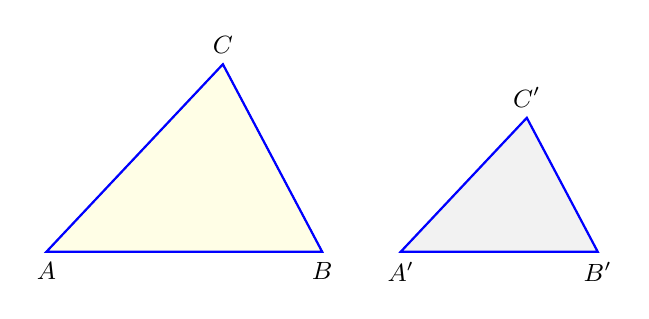
\begin{tikzpicture}[scale=1,font=\small]
\usetikzlibrary{calc}

\begin{scope}[scale=1.4]
\coordinate (a) at (0,0);
\coordinate (c) at (1.6,1.7);
\coordinate (b) at (2.5,0);
\draw[fill=yellow!10] (a) -- (b) -- (c) -- cycle;

\draw[thick, blue] (a) node[black, below] {$A$} -- (b) node[black, below] {$B$} -- (c) node[black, above] {$C$} -- cycle;

\end{scope}

\begin{scope}[xshift=4.5cm, scale=1]
\coordinate (a) at (0,0);
\coordinate (c) at (1.6,1.7);
\coordinate (b) at (2.5,0);
\draw[fill=gray!10] (a) -- (b) -- (c) -- cycle;

\draw[thick, blue] (a) node[black, below] {$A'$} -- (b) node[black, below] {$B'$} -- (c) node[black, above] {$C'$} -- cycle;

\end{scope}


\end{tikzpicture}

\end{figure*}

\begin{proof}
Dall'ipotesi, applicando la proprietà del comporre si ha 
$(AB+AC+BC):AB=(A'B'+A'C'+B'C'):A'B'$ e permutando i medi si ottiene 
la tesi $(AB+AC+BC):(A'B'+A'C'+B'C')=AB:A'B'$.
\end{proof}

\begin{teorema}\label{teo:6.4}% teorema 2
Il rapporto tra le aree\footnotemark{} di due triangoli simili è 
uguale al quadrato del rapporto di similitudine.
\end{teorema}

\footnotetext{una definizione più rigorosa dell'area di un poligono 
verrà data nel capitolo seguente.}

\noindent Ipotesi: $AB:A'B'=AC:A'C'=BC:B'C'$.\tab Tesi: 
$A_{ABC}=A_{A'B'C'}=\overline{AB}^2:\overline{A'B'}^2$.

\begin{figure*}[!htb]
	\centering% Copyright (c) 2015 Daniele Masini - d.masini.it@gmail.com

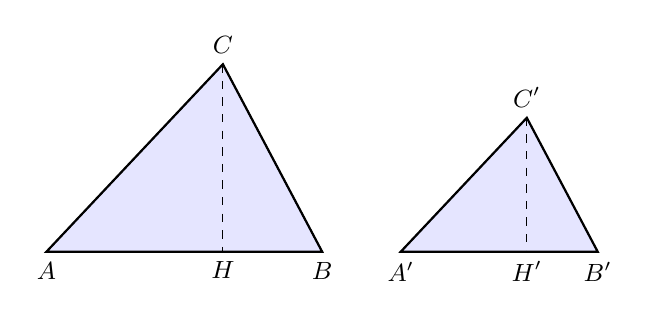
\begin{tikzpicture}[scale=1,font=\small]
\usetikzlibrary{calc}

\begin{scope}[scale=1.4]
\coordinate (a) at (0,0);
\coordinate (c) at (1.6,1.7);
\coordinate (b) at (2.5,0);
\draw[fill=blue!10] (a) -- (b) -- (c) -- cycle;

\draw[thick] (a) node[below] {$A$} -- (b) node[below] {$B$} -- (c) node[above] {$C$} -- cycle;
\draw[dashed] (c) -- ($(a)!(c)!(b)$) node[below] {$H$};

\end{scope}

\begin{scope}[xshift=4.5cm, scale=1]
\coordinate (a) at (0,0);
\coordinate (c) at (1.6,1.7);
\coordinate (b) at (2.5,0);
\draw[fill=blue!10] (a) -- (b) -- (c) -- cycle;

\draw[thick] (a) node[below] {$A'$} -- (b) node[below] {$B'$} -- (c) node[above] {$C'$} -- cycle;
\draw[dashed] (c) -- ($(a)!(c)!(b)$) node[below] {$H'$};

\end{scope}


\end{tikzpicture}

\end{figure*}

\begin{proof}
Prendiamo come riferimento la figura, sappiamo che 
$A_{ABC}=\frac{1}{2}\overline{AB}\cdot\overline{CH}$ e 
$A_{A'B'C'}=\frac{1}{2}\overline{A'B'}\cdot{C'H'}$ quindi 
$\dfrac{A_{ABC}}{A_{A'B'C'}} = 
\dfrac{\overline{AB}\cdot\overline{CH}}{\overline{A'B'}\cdot\overline{
C'H'}} = \dfrac{\overline{AB}}{\overline{A'B'}}\cdot 
\dfrac{\overline{CH}}{\overline{C'H'}}$.
Per quanto stabilito al primo punto di questo paragrafo, il rapporto 
tra le altezze è uguale al rapporto tra le basi: 
$\dfrac{A_{ABC}}{A_{A'B'C'}} = 
\dfrac{\overline{AB}}{\overline{A'B'}}\cdot 
\dfrac{\overline{AB}}{\overline{A'B'}} = 
\dfrac{\overline{AB}^2}{\overline{A'B'}^2}$.
\end{proof}


\section{Similitudine tra poligoni}\label{sect:similitudine_poligoni}

\begin{teorema}
Dati due poligoni simili, le diagonali uscenti da uno stesso vertice 
li decompongono in triangoli ordinatamente simili.
\end{teorema}

\noindent Ipotesi: $ABCDE\sim A'B'C'D'E'$.\tab Tesi: $ABC\sim 
A'B'C'$; $ACE\sim A'C'E'$; $ECD\sim E'C'D'$.

\begin{figure*}[!htb]
	\centering% Copyright (c) 2015 Daniele Masini - d.masini.it@gmail.com

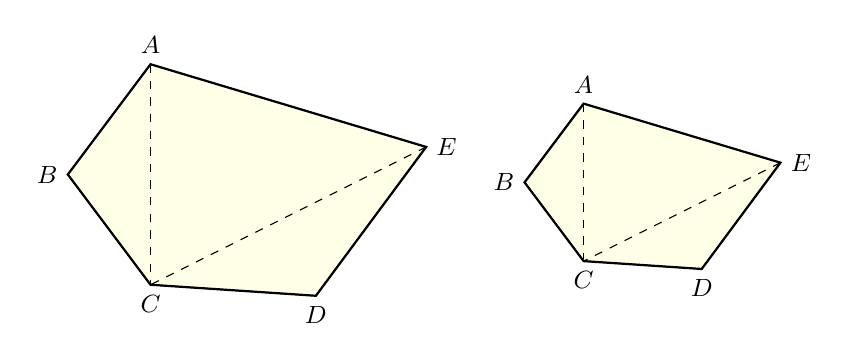
\begin{tikzpicture}[scale=1,font=\small]
\usetikzlibrary{calc}

\begin{scope}[scale=1.4]
\coordinate (a) at (0,0);
\coordinate (b) at (-.75,-1);
\coordinate (c) at (0,-2);
\coordinate (d) at (1.5,-2.1);
\coordinate (e) at (2.5,-0.75);
\draw[fill=yellow!10] (a) -- (b) -- (c) -- (d) -- (e) -- cycle;

\draw[dashed] (a) -- (c);
\draw[dashed] (e) -- (c);
\draw[thick] (a) node[above] {$A$} -- (b) node[left] {$B$} -- (c) node[below] {$C$} -- (d) node[below] {$D$} -- (e) node[right] {$E$} -- cycle;

\end{scope}

\begin{scope}[xshift=5.5cm, yshift=-0.5cm, scale=1]
\coordinate (a) at (0,0);
\coordinate (b) at (-.75,-1);
\coordinate (c) at (0,-2);
\coordinate (d) at (1.5,-2.1);
\coordinate (e) at (2.5,-0.75);
\draw[fill=yellow!10] (a) -- (b) -- (c) -- (d) -- (e) -- cycle;

\draw[dashed] (a) -- (c);
\draw[dashed] (e) -- (c);
\draw[thick] (a) node[above] {$A$} -- (b) node[left] {$B$} -- (c) node[below] {$C$} -- (d) node[below] {$D$} -- (e) node[right] {$E$} -- cycle;

\end{scope}


\end{tikzpicture}

\end{figure*}

\begin{proof}
Ricordiamo che due poligoni si dicono simili se hanno tutti gli 
angoli congruenti e tutti i lati ordinatamente in proporzione. 
Consideriamo, ad esempio, i due pentagoni simili della figura; 
tracciamo le diagonali $CE$, $CA$ e le corrispondenti $C'E'$, $C'A'$. 
Confrontiamo i triangoli $ABC$ e $A'B'C'$; essi sono simili per il 
secondo criterio in quanto hanno due lati in proporzione $AB : A'B' = 
BC : B'C'$ e l'angolo in $B$ congruente a quello in $B'$. Possiamo 
quindi scrivere la proporzione tra i lati omologhi $AB : A'B' = AC : 
A'C'$ e dedurre che $B\widehat{A}C\cong B'\widehat{A'}C'$. Dalla 
similitudine dei due poligoni deduciamo che $C\widehat{A}E\cong 
C'\widehat{A'}E'$ perché differenze di angoli congruenti, e dalla 
proporzione $AB:A'B'=AE:A'E'$, confrontata con la precedente, 
deduciamo la proporzione $AC:A'C'=AE:A'E'$. Consideriamo a questo 
punto i triangoli $ACE$ e $A'C'E'$; anch'essi sono simili per il 
secondo criterio. Ragionando in modo analogo si dimostra la 
similitudine dell'ultima coppia di triangoli.
\end{proof}

\subsection{Similitudine tra poligoni regolari}

Ricordiamo che un poligono si definisce regolare quando ha tutti i 
lati e tutti gli angoli congruenti e che la somma degli angoli 
interni di un poligono qualsiasi è pari a tanti angoli piatti quanti 
sono i lati meno due. Sono poligoni regolari il triangolo equilatero, 
il quadrato, il pentagono regolare, l'esagono regolare, \ldots{} 
Pertanto, affinché due poligoni regolari siano simili è sufficiente 
che abbiano lo stesso numero di lati. Difatti, due poligoni regolari 
con lo stesso numero di lati avranno tutti gli angoli congruenti tra 
loro ed i lati in proporzione, in quanto il rapporto tra due lati 
omologhi qualsiasi sarà sempre lo stesso.

\begin{teorema}
I perimetri di due poligoni regolari dello stesso numero di lati 
stanno tra loro come i rispettivi raggi e come i rispettivi apotemi.
\end{teorema}

% la definizione di raggio di un poligono e di apotema non è mai 
stata data !!!!
Ricordiamo che si chiama raggio di un poligono regolare il raggio 
della circonferenza ad esso circoscritta e che si chiama apotema il 
raggio della circonferenza ad esso inscritta. Poiché in un poligono 
regolare è sempre possibile inscrivere una circonferenza e 
circoscriverne un'altra (vedi i teoremi dimostrati nel 
capitolo~\ref{chap:circonferenza}), questo teorema vale per tutti i 
poligoni regolari con lo stesso numero di lati e quindi simili.

Consideriamo, ad esempio, due pentagoni regolari: $ABCDE$ e 
$A'B'C'D'E'$

\noindent Ipotesi: $ABCDE\sim A'B'C'D'E'$.\\
Tesi: $2p : 2p' = r : r'$, $2p : 2p' = a : a'$ (dove $r$ ed $r'$ sono 
i raggi, $a$ e $a'$ gli apotemi).

\begin{figure*}[!htb]
	\centering% Copyright (c) 2015 Daniele Masini - d.masini.it@gmail.com

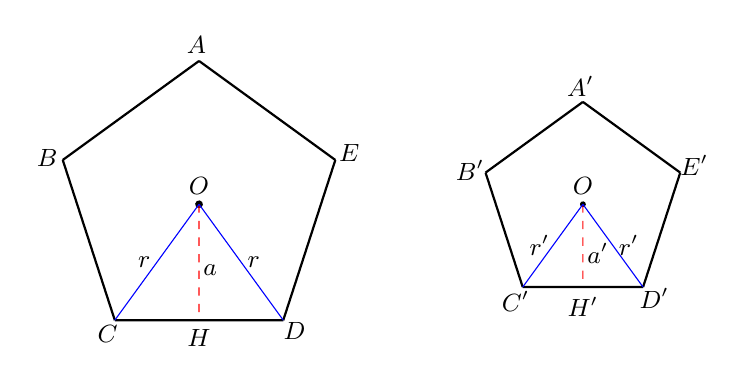
\begin{tikzpicture}[scale=0.65,font=\small]
\usetikzlibrary{calc}
\pgfmathsetmacro{\lati}{5}
\pgfmathsetmacro{\angoloc}{360/\lati}

\begin{scope}[scale=1.4, rotate={\angoloc/2-90}]
%\clip (-2.1,-2.1) rectangle (2.5,2.1);
\coordinate (o) at (0,0);

\foreach \x/\y in {0/D,1/E,2/A,3/B,4/C}
{
	\draw[thick] +({\x*\angoloc}:2) node [shift={({\x*\angoloc-45}:.2)}] {$\y$} -- ({(\x+1)*\angoloc}:2);
}

\draw[fill] (o) circle (1.3pt) node[above] {$O$};

\draw[red, dashed] (o) -- node[black, midway, shift={((0.14,-0.1)}] {$a$} ({(4*\angoloc)+\angoloc/2}:2{*cos(\angoloc/2)}) node[black, below] {$H$};
\draw[blue] (o) -- node[black, midway, shift={((-0.16,0)}] {$r$} ({4*\angoloc}:2);
\draw[blue] (o) -- node[black, midway, shift={((0.16,0)}] {$r$} ({5*\angoloc}:2);

\end{scope}


\begin{scope}[xshift=7.5cm, scale=1, rotate={\angoloc/2-90}]
%\clip (-2.1,-2.1) rectangle (2.5,2.1);
\coordinate (o) at (0,0);

\foreach \x/\y in {0/D,1/E,2/A,3/B,4/C}
{
	\draw[thick] +({\x*\angoloc}:2) node [shift={({\x*\angoloc-45}:.2)}] {$\y'$} -- ({(\x+1)*\angoloc}:2);
}

\draw[fill] (o) circle (1.3pt) node[above] {$O$};

\draw[red, dashed] (o) -- node[black, midway, shift={((0.19,-0.1)}] {$a'$} ({(4*\angoloc)+\angoloc/2}:2{*cos(\angoloc/2)}) node[black, below] {$H'$};
\draw[blue] (o) -- node[black, midway, shift={((-0.17,0)}] {$r'$} ({4*\angoloc}:2);
\draw[blue] (o) -- node[black, midway, shift={((0.2,0)}] {$r'$} ({5*\angoloc}:2);

\end{scope}


\end{tikzpicture}

\end{figure*}

\begin{proof}
Innanzitutto ricordiamo che in due poligoni simili i perimetri stanno 
tra loro come due lati omologhi, quindi avremo ad esempio che
\begin{equation}\label{eq:6.1}
2p : 2p' = CD : C'D'
\end{equation}

Congiungiamo il centro $O$ della circonferenza (sia di quella 
inscritta sia di quella circoscritta) con i due vertici $C$ e $D$ e 
congiungiamo $O'$ con i vertici $C'$ e $D'$. I triangoli isosceli 
$COD$ e $C'O'D'$ sono simili, in quanto l'angolo in $O$ è congruente 
all'angolo in $O'$ (entrambi sono un quinto dell'angolo giro) e gli 
angoli alla base sono congruenti perché ciascuno è metà di un angolo 
congruente, quindi, per il primo criterio di similitudine, sono 
simili. Possiamo allora scrivere la proporzione $CD : C'D' = CO : 
C'O'$.
Poiché $CO = r$ e $C'O' = r'$; tenendo presente la (\ref{eq:6.1}) ed 
applicando la proprietà transitiva dell'uguaglianza possiamo dunque 
scrivere $2p : 2p' = r : r'$. Abbiamo così dimostrato che i perimetri 
dei due poligoni stanno tra loro come i rispettivi raggi.

Ora applichiamo ai due triangoli simili $COD$ e $C'O'D'$ il teorema 
secondo cui in due triangoli simili le altezze sono proporzionali 
alle rispettive basi $OH : O'H' = CD : C'D'$. Applicando anche questa 
volta la proprietà transitiva della congruenza e ponendo $OH = a$ e 
$O'H' =a'$, avremo $2p : 2p' = a : a'$.
Quindi i perimetri dei due poligoni stanno tra loro come i rispettivi 
apotemi.
\end{proof}

Il lettore dimostri da solo, ricorrendo ai teoremi precedenti, che le 
aree di due poligoni regolari dello stesso numero di lati stanno tra 
loro come i quadrati costruiti sui rispettivi raggi o apotemi.


\section{Proprietà di secanti e tangenti ad una 
circonferenza}\label{sect:proprieta_secanti_tangenti}

Osserviamo che in una circonferenza, due corde possono intersecarsi 
internamente al cerchio o esternamente.
\begin{teorema}[delle corde]
Se due corde di una circonferenza si incontrano in un punto interno 
al cerchio allora le due corde restano divise in modo che le parti di 
una siano i medi e le parti dell'altra gli estremi della stessa 
proporzione.
\end{teorema}

\noindent Ipotesi: $AB$ e $CD$ sono due corde che si intersecano in 
$E$.\tab Tesi: $EB:ED=EC:EA$.

\noindent\begin{minipage}{0.65\textwidth}\parindent15pt
\begin{proof}
Dovendo arrivare ad una proporzione tra segmenti, cercheremo di 
individuare la similitudine tra due triangoli; a questo scopo 
congiungiamo $B$ con $C$ e $A$ con $D$. Consideriamo i triangoli 
\ldots\ldots{} ed \ldots\ldots{} Essi hanno: 
$\ldots\ldots{}\cong\ldots\ldots{}$ perché opposti al vertice, 
$C\widehat{B}A\cong C\widehat{D}A$ perché insistono 
\ldots\ldots\ldots{} Dunque risultano simili per il primo criterio di 
similitudine. Quindi, individuati i lati omologhi, possiamo scrivere 
la proporzione $BC:DA=EB:ED=EC:EA$.
\end{proof}
\end{minipage}\hfil
\begin{minipage}{0.35\textwidth}
	\centering% Copyright (c) 2015 Daniele Masini - d.masini.it@gmail.com

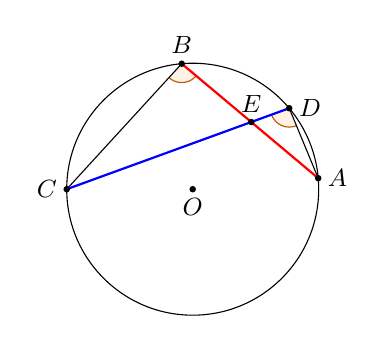
\begin{tikzpicture}[scale=0.8,font=\small]
\usetikzlibrary{calc}

\begin{scope}

\coordinate (a) at (5:2);
\coordinate (b) at (95:2);
\coordinate (c) at (180:2);
\coordinate (d) at (40:2);
\coordinate (o) at (0,0);

\draw (o) circle (2);
\draw[fill] (o) circle (1.2pt) node[below] {$O$};

\coordinate (e) at (intersection of a--b and c--d);

\begin{scope}
\clip (c)--(b)--(e) -- cycle;
\draw[orange!70!black, fill=orange!10] (b) circle (0.3);
\end{scope}
\begin{scope}
\clip (a)--(d)--(e) -- cycle;
\draw[orange!70!black, fill=orange!10] (d) circle (0.3);
\end{scope}


\draw (c) -- (b);
\draw (a) -- (d);

\draw[thick, red] (a) -- (b);
\draw[thick, blue] (c) -- (d);
\draw[fill] (a) circle (1.2pt) node[right] {$A$};
\draw[fill] (b) circle (1.2pt) node[above] {$B$};
\draw[fill] (c) circle (1.2pt) node[left] {$C$};
\draw[fill] (d) circle (1.2pt) node[right] {$D$};
\draw[fill] (e) circle (1.2pt) node[above] {$E$};

\end{scope}

\end{tikzpicture}

\end{minipage}\vspace{5pt}

\begin{teorema}[delle secanti]
Se da un punto esterno a un cerchio si conducono due secanti alla 
circonferenza, allora un'intera secante e la sua parte esterna 
formano i medi e l'altra secante e la sua parte esterna sono gli 
estremi di una stessa proporzione.
\end{teorema}

\noindent Ipotesi: $AB$ e $CD$ sono due corde che si intersecano in 
$E$ esterno alla circonferenza.\tab Tesi: $EC:ED=EA:EB$.

\noindent\begin{minipage}{0.65\textwidth}\parindent15pt
\begin{proof}
Dovendo determinare una proporzione tra segmenti, cercheremo di 
individuare la similitudine tra due triangoli; a questo scopo 
congiungiamo $B$ con $C$ e $A$ con $D$. I triangoli $EBC$ ed $EAD$ 
sono simili perché hanno: $B\widehat{E}C\cong D\widehat{E}A$ in 
comune, $B\widehat{C}E\cong D\widehat{A}E$ perché insistono sullo 
stesso arco $DB$. Risultano quindi simili per il primo criterio di 
similitudine. Possiamo allora scrivere la proporzione tra i lati 
$EC:ED=EA:EB$.
\end{proof}
\end{minipage}\hfil
\begin{minipage}{0.35\textwidth}
	\centering% Copyright (c) 2015 Daniele Masini - d.masini.it@gmail.com

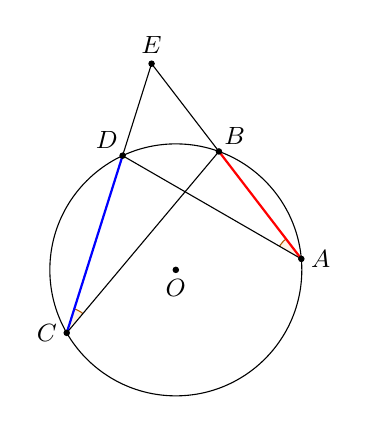
\begin{tikzpicture}[scale=0.8,font=\small]
\usetikzlibrary{calc}

\begin{scope}

\coordinate (a) at (5:2);
\coordinate (b) at (70:2);
\coordinate (c) at (210:2);
\coordinate (d) at (115:2);
\coordinate (o) at (0,0);

\draw (o) circle (2);
\draw[fill] (o) circle (1.2pt) node[below] {$O$};

\coordinate (e) at (intersection of a--b and c--d);

\begin{scope}
\clip (c)--(b)--(e) -- cycle;
\draw[orange!70!black, fill=orange!10] (c) circle (0.4);
\end{scope}
\begin{scope}
\clip (a)--(d)--(e) -- cycle;
\draw[orange!70!black, fill=orange!10] (a) circle (0.4);
\end{scope}


\draw (c) -- (b);
\draw (a) -- (d);
\draw (d) -- (e);
\draw (b) -- (e);

\draw[thick, red] (a) -- (b);
\draw[thick, blue] (c) -- (d);
\draw[fill] (a) circle (1.2pt) node[right] {$A$};
\draw[fill] (b) circle (1.2pt) node[shift={(0.2,0.2)}] {$B$};
\draw[fill] (c) circle (1.2pt) node[left] {$C$};
\draw[fill] (d) circle (1.2pt) node[shift={(-0.2,0.2)}] {$D$};
\draw[fill] (e) circle (1.2pt) node[above] {$E$};

\end{scope}

\end{tikzpicture}

\end{minipage}\vspace{5pt}

\begin{teorema}[della secante e della tangente]
Se da un punto esterno a un cerchio si conduce una secante e una 
tangente alla circonferenza, allora il segmento di tangente è medio 
proporzionale tra l'intera secante e la sua parte esterna alla 
circonferenza.
\end{teorema}

\noindent Ipotesi: $B$ punto esterno alla circonferenza, $BA$ 
tangente in $A$, $BE$ secante in $D$ ed $E$.\tab Tesi: $BE:BA=BA:BD$.

\noindent\begin{minipage}{0.65\textwidth}\parindent15pt
\begin{proof}
Dovendo determinare una proporzione tra segmenti, cercheremo di 
individuare la similitudine tra due triangoli; a questo scopo 
congiungiamo $A$ con $E$ e $A$ con $D$ e consideriamo i triangoli 
$EBA$ e $DBA$. Essi hanno $E\widehat{B}A\cong D\widehat{B}A$ perché 
coincidenti, $B\widehat{E}A\cong D\widehat{B}A$ perché angoli alla 
circonferenza che insistono sullo stesso arco $AC$. I due triangoli 
sono simili per il primo criterio di similitudine. Individuati i lati 
omologhi si può scrivere la proporzione $BE:BA=BA:BD$.
\end{proof}
\end{minipage}\hfil
\begin{minipage}{0.35\textwidth}
	\centering% Copyright (c) 2015 Daniele Masini - d.masini.it@gmail.com

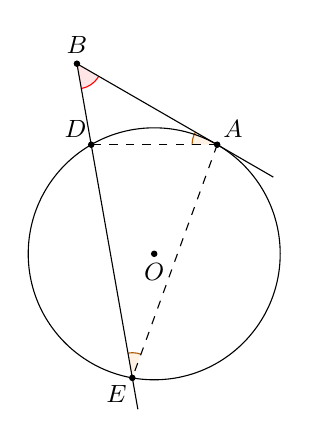
\begin{tikzpicture}[scale=0.8,font=\small]
\usetikzlibrary{calc}

\begin{scope}

\coordinate (a) at (60:2);
\path (a) -- +(150:3) coordinate (b1);
\coordinate (d) at (120:2);
\coordinate (e) at (260:2);
\coordinate (o) at (0,0);

\draw[fill] (o) circle (1.2pt) node[below] {$O$};

\coordinate (b) at (intersection of e--d and a--b1);

\begin{scope}
\clip (a)--(b)--(d) -- cycle;
\draw[orange!70!black, fill=orange!10] (a) circle (0.4);
\draw[red, fill=red!10] (b) circle (0.4);
\end{scope}
\begin{scope}
\clip (a)--(d)--(e) -- cycle;
\draw[orange!70!black, fill=orange!10] (e) circle (0.4);
\end{scope}

\draw (o) circle (2);

\draw ($(a)!-0.4!(b)$) -- (b);
\draw ($(e)!-0.1!(b)$) -- (b);
\draw[dashed] (a) -- (d);
\draw[dashed] (a) -- (e);

\draw[fill] (a) circle (1.2pt) node[shift={(0.2,0.2)}] {$A$};
\draw[fill] (b) circle (1.2pt) node[above] {$B$};
\draw[fill] (d) circle (1.2pt) node[shift={(-0.2,0.2)}] {$D$};
\draw[fill] (e) circle (1.2pt) node[shift={(-0.2,-0.2)}] {$E$};

\end{scope}

\end{tikzpicture}

\end{minipage}\vspace{5pt}

\section{La sezione aurea}\label{sect:sezione_aurea}

\begin{definizione}
La \emph{sezione aurea} di un segmento $AB$ è quella parte $AC$ del 
segmento media proporzionale tra l'intero segmento e la parte 
rimanente $CB$.
\end{definizione}


\begin{inaccessibleblock}[Figura: TODO]
 \begin{figure}[!htb]
	\centering% Copyright (c) 2015 Daniele Masini - d.masini.it@gmail.com

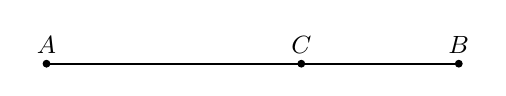
\begin{tikzpicture}[scale=1,font=\small]
\usetikzlibrary{calc}

\begin{scope}

% sez. aurea è a/b:   b:a=a:(a+b)  -> a/b = (1+sqrt(5))/2

\coordinate (a) at (0,0);
\coordinate (c) at ({2*(1+sqrt(5))/2},0);
\coordinate (b) at ({2*(1+sqrt(5))/2+2},0);

\draw[thick] (a) -- (b);

\draw[fill] (a) circle (1.2pt) node[above] {$A$};
\draw[fill] (b) circle (1.2pt) node[above] {$B$};
\draw[fill] (c) circle (1.2pt) node[above] {$C$};

\end{scope}

\end{tikzpicture}
	\caption{$AC$ è la sezione aurea del segmento 
$AB$}\label{fig:sez_aurea}
\end{figure}
\end{inaccessibleblock}

In riferimento alla figura~\ref{fig:sez_aurea} si ha $AB : AC = AC : 
CB$.

\subsection{Il punto di vista algebrico}

Dato un qualunque segmento $AB$ di misura $a$, è sempre possibile 
determinare su di esso il punto $C$ tale che valga la proporzione $AB 
: AC = AC : CB$?

La risposta è affermativa. Infatti, poniamo 
$\overline{AC}=x\:\Rightarrow\:\overline{CB}=a-x$ e riscriviamo la 
proporzione passando alle misure: $a : x = x : (a-x)$.
Per la proprietà fondamentale delle proporzioni numeriche si ottiene 
$x^2=a(a-x)$, da cui  sviluppando i calcoli si ha l'equazione di 
secondo grado $x^2+ax-a^2=0$ che ha discriminante $5a^2$, positivo 
per qualunque $a$. Quindi l'equazione ammette due soluzioni, di cui 
una negativa che va scartata. Rimane la soluzione 
$x=a\dfrac{-1+\sqrt{5}}{2}$, positiva poiché $a>0$.

\subsection{Il punto di vista geometrico}

Possiamo determinare la sezione aurea di un segmento con una 
costruzione geometrica?

La risposta è positiva. La costruzione che riportiamo è quella di 
Eulero, che sfrutta il teorema della tangente e della secante.
La costruzione, riportata in figura~\ref{fig:sez_aurea2}, si compone 
dei passi passi sotto descritti (per riprodurla si può anche 
utilizzare un software di geometria dinamica come \emph{Geogebra}):

\begin{enumerate*}
\item si disegni un segmento $AB$;
\item si tracci la retta $p$, perpendicolare ad $AB$ e passante per 
$B$;
\item si disegni la circonferenza $\gamma_1$ di centro $B$ e raggio 
$AB$;
\item sia $H$ uno dei punti di intersezione della retta $p$ con 
$\gamma_1$;
\item sia $M$ il punto medio di $BH$;
\item si disegni la circonferenza $\gamma_2$ di centro $M$ e raggio 
$MB$;
\item si tracci la retta $AM$;
\item siano $P$ ed $E$ i punti di intersezione della retta $AM$ con 
la circonferenza $\gamma_2$ (sia $P$ quello più vicino ad $A$);
\item si tracci la circonferenza $\gamma_3$ di centro $A$ e raggio 
$AP$;
\item sia $C$ il punto di intersezione di $\gamma_3$ con $AB$.
\end{enumerate*}


\begin{inaccessibleblock}[Figura: TODO]
 \begin{figure}[!htb]
	\centering% Copyright (c) 2015 Daniele Masini - d.masini.it@gmail.com

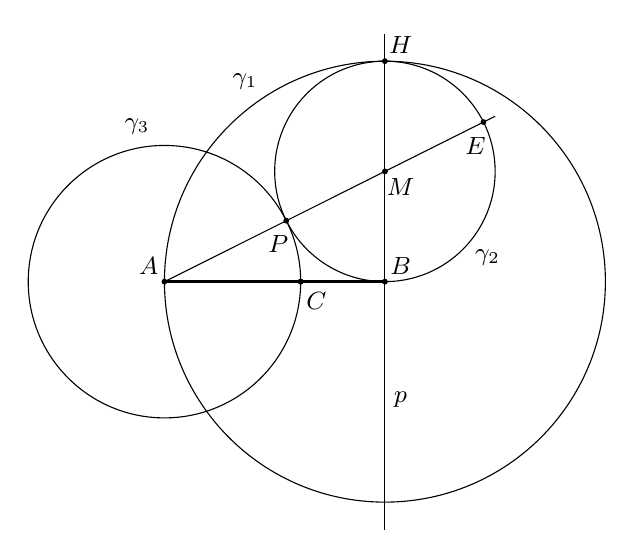
\begin{tikzpicture}[scale=0.7,font=\small]
\usetikzlibrary{calc, intersections}

\begin{scope}

\coordinate (a) at (0,0);
%\coordinate (c) at ({2*(1+sqrt(5))/2},0);
\coordinate (b) at (4,0);

\path[name path=SegmBase] (a) -- (b); 
\draw[name path=Circle1] (b) circle (4) node [shift={(125:3.1)}] {$\gamma_1$};
\draw[name path=Retta1] (4,-4.5) -- node [shift={(.2,-1.5)}] {$p$} (4,4.5);
\path [name intersections={of=Circle1 and Retta1}] ;
\draw[fill] (intersection-1) coordinate (h) circle (1.2pt) node[shift={(.2,.2)}] {$H$};
\coordinate (m) at ($(b)!0.5!(h)$);
\draw[name path=Circle2] (m) circle (2) node [shift={(-40:1.7)}] {$\gamma_2$};
\draw[name path=Retta2] (a) -- ($(a)!1.5!(m)$);
\path [name intersections={of=Circle2 and Retta2}] ;
\draw[fill] (intersection-2) coordinate (p) circle (1.2pt) node[shift={(-.1,-.3)}] {$P$};
\draw[fill] (intersection-1) coordinate (e) circle (1.2pt) node[shift={(-.1,-.3)}] {$E$};
\draw[name path=Circle3] (a) let \p1=($(p)-(a)$) in circle ({veclen(\x1,\y1)}) node [shift={(100:2)}] {$\gamma_3$};
\path [name intersections={of=Circle3 and SegmBase}] ;
\draw[fill] (intersection-1) coordinate (c) circle (1.2pt);

\draw[very thick] (a) -- (b);

\draw[fill] (a) circle (1.2pt) node[shift={(-.2,.2)}] {$A$};
\draw[fill] (b) circle (1.2pt) node[shift={(.2,.2)}] {$B$};
\draw[fill] (c) circle (1.2pt) node[shift={(.2,-.25)}] {$C$};
\draw[fill] (m) circle (1.2pt) node[shift={(.2,-.2)}] {$M$};

\end{scope}

\end{tikzpicture}

	\caption{Costruzione della sezione aurea $AC$ di 
$AB$}\label{fig:sez_aurea2}
\end{figure}
\end{inaccessibleblock}

Dimostriamo che il segmento $AC$ così costruito è la sezione aurea 
del segmento $AB$.
\begin{proof}
Per costruzione risulta $AB$ tangente a $\gamma_2$ e $AE$ secante, 
quindi per il teorema della tangente e della secante si ha: $AE : AB 
= AB : AP$; per la proprietà dello scomporre $(AE-AB):AB=(AB-AP):AP$.
Per costruzione si sa che: $AB\cong HB\cong PE$ e quindi $AE - AB 
\cong AE - PE\cong AP$.
Dal momento che $AP\cong AC$ si ottiene $AB - AP \cong AB - AC \cong 
CB$.
Sostituendo nella proporzione $(AE-AB):AB=(AB-AP):AP$ si ottiene la 
proporzione $AP : AB = CB : AP$.
E infine, applicando la proprietà dell'invertire, si ottiene la tesi 
$AB : AC = AC : CB$.
\end{proof}

\begin{teorema}
ll lato del decagono regolare è la sezione aurea del raggio della 
circonferenza ad esso circoscritta.
\end{teorema}

Detto $OA$ il raggio della circonferenza e $AB$ il lato del decagono 
regolare, si deve dimostrare che: $OA:AB=AB:(OA-AB)$.

\begin{figure*}[!htb]
	\begin{center}
		\begin{minipage}{0.45\textwidth}
			\centering
			% Copyright (c) 2015 Daniele Masini - d.masini.it@gmail.com

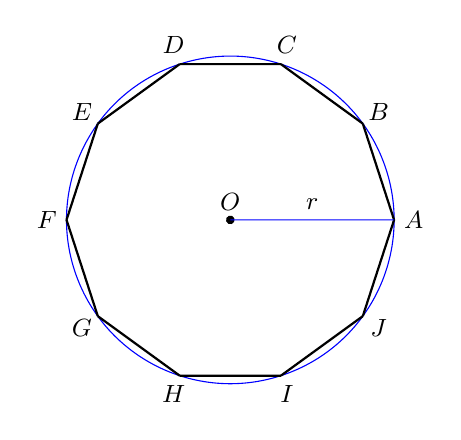
\begin{tikzpicture}[scale=0.65,font=\small]
\usetikzlibrary{calc}
\pgfmathsetmacro{\lati}{10}
\pgfmathsetmacro{\angoloc}{360/\lati}

\begin{scope}[scale=1.6, rotate={\angoloc/2-90}]
%\clip (-2.1,-2.1) rectangle (2.5,2.1);
\coordinate (o) at (0,0);
\draw[blue] (o) circle (2);

\foreach \x/\y in {0/I,1/J,2/A,3/B,4/C,5/D,6/E,7/F,8/G,9/H}
{
	\draw[thick] +({\x*\angoloc}:2) node [shift={({\x*\angoloc-72}:.25)}] {$\y$} -- ({(\x+1)*\angoloc}:2);
}

\draw[fill] (o) circle (1.3pt) node[above] {$O$};

%\draw[red, dashed] (o) -- node[black, midway, shift={((0.14,-0.1)}] {$a$} ({(4*\angoloc)+\angoloc/2}:2{*cos(\angoloc/2)}) node[black, below] {$H$};
\draw[blue] (o) -- node[black, midway, shift={((0,0.2)}] {$r$} ({2*\angoloc}:2);

\end{scope}


\end{tikzpicture}

		\end{minipage}
		\hspace{0.03\textwidth}	
		\begin{minipage}{0.45\textwidth}
			\centering
			% Copyright (c) 2015 Daniele Masini - d.masini.it@gmail.com

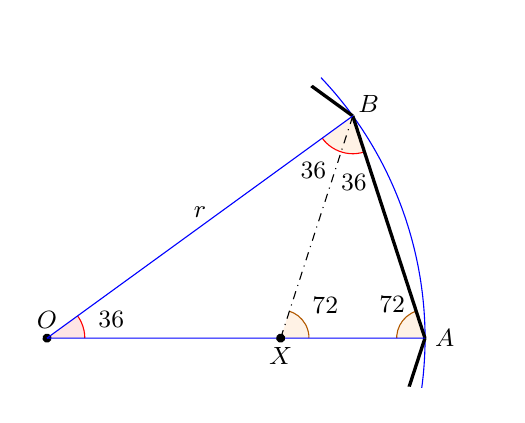
\begin{tikzpicture}[scale=0.8, font=\small]
\usetikzlibrary{calc}
%\pgfmathsetmacro{\grado}{1}
\pgfmathsetmacro{\lati}{10}
\pgfmathsetmacro{\angoloc}{360/\lati}

\begin{scope}[scale=3, rotate={\angoloc/2-90}]
\coordinate (o) at (0,0);

\begin{scope}
\clip ({\angoloc*1.8+180}:0.1) -- ({\angoloc*3.2+180}:0.1) -- ({\angoloc*1.8}:2.4) -- ({\angoloc*3.2}:2.4) -- cycle;
\draw[blue] (o) circle (2);

\foreach \x/\y in {0/D,1/E,2/A,3/B,4/C,5/D,6/E,7/F,8/G,9/H,10/I}
{
	\path +({\x*\angoloc}:2) coordinate (\y);
}

\begin{scope}
\clip (o) -- (B) -- (A) -- cycle;
\draw[red, fill=red!10] (o) circle (0.2) node[black, shift={(0.45*\angoloc:0.85)}] {$36\grado$};
\draw[red, fill=orange!10] (B) circle (0.2) node[black, shift={(270-\angoloc:0.85)}] {$36\grado$} node[black, shift={(307-\angoloc:0.85)}] {$36\grado$};
\draw[orange!70!black, fill=orange!10] (A) circle (0.15) node[black, shift={(170-\angoloc:0.6)}] {$72\grado$};
\end{scope}

\path (B) let \p1 = ($(A)-(B)$) in -- ($(B)!{veclen(\x1,\y1)}!(o)$) -- +($(A)-(B)$) coordinate (b1);
\coordinate (a1) at (intersection of B--b1 and A--o);

\begin{scope}
\clip (a1) -- (B) -- (A) -- cycle;
\draw[orange!70!black, fill=orange!10] (a1) circle (0.15) node[black, shift={(\angoloc:0.7)}] {$72\grado$};
\end{scope}

\draw[dashdotted] (B) -- (a1);

\foreach \x/\y in {0/D,1/E,2/A,3/B,4/C,5/D,6/E,7/F,8/G,9/H,10/I}
{
	\draw[very thick] +({\x*\angoloc}:2) coordinate (\y) node [shift={({\x*\angoloc-72}:.25)}] {$\y$} -- ({(\x+1)*\angoloc}:2);
}

\end{scope}
\draw[fill] (o) circle (0.6pt) node[above] {$O$};

%\draw[red, dashed] (o) -- node[black, midway, shift={((0.14,-0.1)}] {$a$} ({(4*\angoloc)+\angoloc/2}:2{*cos(\angoloc/2)}) node[black, below] {$H$};
\draw[blue] (o) -- ({2*\angoloc}:2);
\draw[blue] (o) -- node [black, above] {$r$} ({3*\angoloc}:2);

\draw[fill] (a1) circle (0.6pt) node[below] {$X$};


\end{scope}


\end{tikzpicture}

		\end{minipage}
	\end{center}
\end{figure*}

\begin{proof}
Quando si congiungono i vertici di un poligono regolare con il centro 
della circonferenza (inscritta o circoscritta) si ottengono tanti 
triangoli isosceli quanti sono i lati, e questi triangoli sono tutti 
congruenti tra loro.
Consideriamo, per il decagono regolare, uno solo di questi triangoli, 
per esempio $AOB$. L'angolo in $O$ vale $36\grado$ (è infatti un 
decimo dell'angolo giro), quindi gli angoli alla base varranno 
ciascuno $\dfrac{180\grado-36\grado}{2} = 72\grado$.

Tracciamo la bisettrice $BX$ dell'angolo $A\widehat{B}O$. Si ottiene 
il triangolo $OBX$ che è isoscele in quanto ha due angoli di 
$36\grado$, ed il triangolo $AXB$ anch'esso isoscele poiché ha due 
angoli di $72\grado$ (l'angolo $A\widehat{B}X$ e l'angolo 
$A\widehat{X}B$).  
Quindi avremo $BX\cong OX\cong AB$.
Inoltre, i triangoli $AOB$ e $ABX$ sono simili in quanto hanno gli 
angoli rispettivamente congruenti.
Si può quindi scrivere la proporzione $OA:AB=AB:AX$, dove il primo 
$AB$ è il lato obliquo del triangolo $ABX$ e il secondo $AB$ è la 
base di $AOB$.
Abbiamo così dimostrato il teorema, in quanto $AX$ è congruente a 
$OA-OX \cong OA-AB$ ($OA\cong OB$ perché raggi della stessa 
circonferenza, $OX\cong AB$ per quanto dimostrato precedentemente).
\end{proof}

Sostituendo alle grandezze le loro misure, chiamando ad esempio $r$ 
il raggio della circonferenza circoscritta ed $l$ il lato del 
decagono regolare, la proporzione diventa $r:l=l:(r-l)$.
Moltiplicando tra loro gli estremi ed i medi, si ha $l^2=r^2-rl 
\:\Rightarrow\: l^2+rl-r^2=0$.
Risolvendo l'equazione rispetto ad $l$ si ha $l=\dfrac{-r\pm 
r\sqrt{5}}{2}$, tenendo conto che è accettabile solo la lunghezza 
positiva, si ottiene $l=r\dfrac{\sqrt{5}-1}{2}$.

\begin{wrapfigure}{r}{0.35\textwidth}
	\centering% Copyright (c) 2015 Daniele Masini - d.masini.it@gmail.com

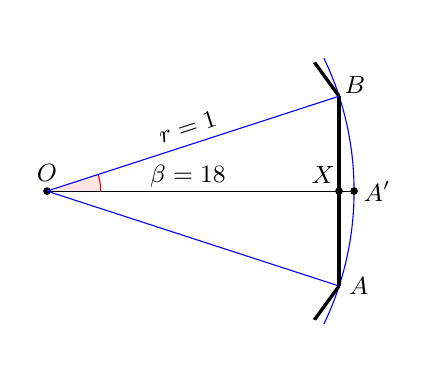
\begin{tikzpicture}[scale=0.65, font=\small]
\usetikzlibrary{calc}
\pgfmathsetmacro{\lati}{10}
\pgfmathsetmacro{\angoloc}{360/\lati}

\begin{scope}[scale=3, rotate={-90}]
\coordinate (o) at (0,0);

\begin{scope}
\clip ({\angoloc*1.8+180}:0.1) -- ({\angoloc*3.2+180}:0.1) -- ({\angoloc*1.8}:2.5) -- ({\angoloc*3.2}:2.5) -- cycle;
\draw[blue] (o) circle (2);

\foreach \x/\y in {0/D,1/E,2/A,3/B,4/C,5/D,6/E,7/F,8/G,9/H,10/I}
{
	\path +({\x*\angoloc}:2) coordinate (\y);
}

\coordinate (ax) at (0,2);
\coordinate (d) at (intersection of B--A and o--ax);

\begin{scope}
\clip (o) -- (B) -- (ax) -- cycle;
\draw[red, fill=red!10] (o) circle (0.35) node[black, shift={(0.17*\angoloc:1.8)}] {$\beta=18\grado$};
\end{scope}

\draw (o) -- (ax);

\foreach \x/\y in {0/D,1/E,2/A,3/B,4/C,5/D,6/E,7/F,8/G,9/H,10/I}
{
	\draw[very thick] +({\x*\angoloc}:2) coordinate (\y) node [shift={({\x*\angoloc-72}:.25)}] {$\y$} -- ({(\x+1)*\angoloc}:2);
}

\end{scope}

\draw[fill] (o) circle (0.6pt) node[above] {$O$};
\draw[fill] (ax) circle (0.6pt) node[right] {$A'$};
\draw[fill] (d) circle (0.6pt) node[shift={(-0.2,0.2)}] {$X$};

%\draw[red, dashed] (o) -- node[black, midway, shift={((0.14,-0.1)}] {$a$} ({(4*\angoloc)+\angoloc/2}:2{*cos(\angoloc/2)}) node[black, below] {$H$};
\draw[blue] (o) -- ({2*\angoloc}:2);
\draw[blue] (o) -- node [black, above, rotate=18] {$r=1$} ({3*\angoloc}:2);

\end{scope}


\end{tikzpicture}

\end{wrapfigure}
Un'importante applicazione di questo teorema è il calcolo del valore 
del seno dell'angolo di $18\grado$.
Considerando la circonferenza goniometrica (di raggio unitario), se 
poniamo l'angolo di $36\grado$ col vertice nell'origine degli assi, 
questo verrà dimezzato dall'asse $x$ e di conseguenza verrà dimezzato 
anche il lato opposto (abbiamo infatti un triangolo isoscele in cui 
la bisettrice dell'angolo al vertice è anche mediana relativa alla 
base).
Il seno di $18\grado$ corrisponde alla lunghezza di $XB$, che è 
quindi metà del lato del decagono regolare, perciò vale $\sin 18\grado 
= \dfrac{\sqrt{5}-1}{4}$.

% \newpage
% 
% \input{./chap/06_esercizi}
% 
% \cleardoublepage
